\documentclass[aps,prb,twocolumn,superscriptaddress,longbibliography,floatfix]{revtex4-2}

\usepackage{amsmath,amssymb}
\usepackage{graphicx}
\usepackage{hyperref}
\usepackage{booktabs}
\usepackage{xcolor}

\begin{document}

\title{Adaptive machine learning of universal scaling parameters for interatomic potentials}

\author{Alastair James Arthur Price}
\affiliation{Department of Chemistry, University of Toronto, Toronto, Ontario M5S 3H6, Canada}
\affiliation{Vector Institute for Artificial Intelligence, Toronto, Ontario M5S 1M1, Canada}

\author{O.~Anatole von Lilienfeld}
\email{anatole.vonlilienfeld@utoronto.ca}
\affiliation{Department of Chemistry, University of Toronto, Toronto, Ontario M5S 3H6, Canada}
\affiliation{Vector Institute for Artificial Intelligence, Toronto, Ontario M5S 1M1, Canada}

\date{\today}

\begin{abstract}
When a known physical equation relates a small number of interpretable parameters to the quantity of interest, machine learning models can achieve better generalization by predicting those parameters rather than the quantity itself. We recently demonstrated this ``adaptive'' strategy for density functionals, where learning the exchange mixing parameter $\alpha$ yields the aPBE0 functional. Here, we demonstrate this principle more generally using interatomic potentials: instead of learning the potential energy surface directly, we train models to predict the universal scaling parameters of known analytical forms, the Rose/UBER parameters $(E_c, r_e, l)$ or Lennard-Jones parameters $(\varepsilon, \sigma)$, and reconstruct the full energy curve via the physics based equations. On synthetic Morse potentials, this adaptive approach yields $2.3\times$ lower extrapolation error than direct learning; for Lennard-Jones potentials on a fixed radial grid, the advantage reaches $42\times$. Validation was undertaken on 30 DFT diatomic binding curves (PBE/def2-SVP) confirms the advantage exists on real quantum-chemical data: $1.15\times$ for interpolation and $1.74\times$ for extrapolation to unseen elements. The adaptive machine learning approach also provides analytical forces at no additional cost, and a delta learning extension yields a further $2.7\times$ improvement. Together with aPBE0, these results establish adaptive parameter learning as a general strategy for physics-informed machine learning across computational chemistry.
\end{abstract}

\maketitle


%=============================================================================
\section{Introduction}
\label{sec:intro}
%=============================================================================

A recurring challenge in scientific machine learning is extrapolation: models that interpolate accurately within their training domain often fail catastrophically on unseen systems. This problem is not specific to any application and it arises whenever a flexible model (neural network, kernel method, linear expansion) is asked to predict outside the range of its training data. The underlying issue is structural: without physical constraints, nothing prevents the model from producing unphysical behaviour in unexplored regions.

We recently proposed a general strategy to address this: \emph{adaptive parameter learning}. Rather than training a model to predict the physical quantity of interest directly, one trains it to predict the parameters of a known physics equation, which then produces the output with built-in physical constraints. In the context of density functional theory, this strategy led to the adaptive PBE0 functional approach (aPBE0)~\cite{Khan2025}, where a machine learning model predicts the exchange mixing fraction $\alpha$ from electron density descriptors rather than learning the exchange-correlation energy $E_\mathrm{xc}$ directly. The basic physics equation $E_\mathrm{xc} = (1-\alpha)E_\mathrm{PBE} + \alpha E_\mathrm{HF}$ then enforces correct functional behaviour even when outside the training distribution.

The key insight is that the parameters $\alpha$, $E_c$, $\varepsilon$, or $\sigma$ are bounded, smooth, and low-dimensional, making them inherently easier regression targets than the quantities they parameterize directly. In this work, we demonstrate that the same adaptive principle extends naturally from density functionals to interatomic potentials: we train models to predict the universal scaling parameters of known analytical forms and reconstruct the full potential energy curve via a physics based equation.

Machine learning interatomic potentials (MLIPs) provide a natural test bed for this strategy. Neural network potentials~\cite{Behler2007,Smith2017}, Gaussian approximation potentials~\cite{Bartok2010,Deringer2019}, atomic cluster expansion models~\cite{Drautz2019}, and equivariant message-passing architectures~\cite{Batatia2022} have achieved remarkable performance within their training domains~\cite{Unke2021}, yet a consistent isssue arises for all, they extrapolate poorly to configurations far from the training distribution~\cite{Zuo2020,Noe2020}. Kernel-based models employ radial basis function kernels that decay to zero far from training points, causing predictions to collapse to the training mean,~\cite{Bartok2010} and neural networks, lacking physical constraints on their asymptotic behaviour, can produce unphysical energies and forces in unexplored regions of the configuration space.

For interatomic potentials, the adaptive approach exploits the well-established and understood universality of binding energy curves. The Rose/UBER (universal binding energy relation) equation~\cite{Rose1984,Ferrante1983} describes covalent and metallic bonding with three basic parameters: the cohesive energy $E_c$, equilibrium distance $r_e$, and length scale $l$. The Lennard-Jones potential~\cite{LennardJones1924} describes van der Waals interactions with the well depth $\varepsilon$ and size parameter $\sigma$. Our approach is further motivated by Euler's homogeneous function theorem, which provides exact constraints for power-law potentials but fails for realistic bonding interactions. The non-homogeneity of Morse~\cite{Morse1929} and Lennard-Jones potentials indicates that no single power law describes the interaction at all separations, yet when expressed in scaled coordinates, their binding curves collapse onto universal forms, confirming that the material-specific information is encoded in a small number of scaling parameters.

Here we demonstrate the adaptive approach on three systems of increasing complexity: (i) synthetic Morse potentials fitted to the Rose/UBER equation, (ii) Lennard-Jones potentials on a fixed radial grid, and (iii) DFT binding curves for 30 diatomic molecules. In all cases, the adaptive approach outperforms direct learning for extrapolation, with advantages ranging from $1.7\times$ to $42\times$ depending on the system and extrapolation required for the task.


%=============================================================================
\section{Theory}
\label{sec:theory}
%=============================================================================

%-----------------------------------------------------------------------------
\subsection{Euler's theorem and the virial relation}
\label{sec:euler}
%-----------------------------------------------------------------------------

A scalar function $f(\mathbf{x})$ is homogeneous of degree $d$ if $f(s\mathbf{x}) = s^d f(\mathbf{x})$ for all $s > 0$. Euler's theorem states that such functions satisfy
\begin{equation}
  \mathbf{x} \cdot \nabla f = d\, f(\mathbf{x}).
  \label{eq:euler}
\end{equation}
For a radial pair potential $V(r)$, this reduces to the virial relation
\begin{equation}
  r\, F(r) = -d\, V(r),
  \label{eq:virial}
\end{equation}
where $F = -dV/dr$ is the force.

Equation~\eqref{eq:virial} holds exactly for power-law potentials: the Coulomb interaction ($V \propto r^{-1}$, $d = -1$) and London dispersion ($V \propto r^{-6}$, $d = -6$). A plot of $rF$ versus $V$ (the ``virial plot'') yields a straight line with slope $-d$ for any homogeneous potential [Fig.~\ref{fig:virial}(a,b)].

%-----------------------------------------------------------------------------
\subsection{Non-homogeneity of realistic potentials}
\label{sec:nonhomo}
%-----------------------------------------------------------------------------

Realistic covalent and van der Waals potentials are not homogeneous. The Morse potential~\cite{Morse1929},
\begin{equation}
  V_\mathrm{Morse}(r) = D_e \bigl(1 - e^{-a(r - r_e)}\bigr)^2,
  \label{eq:morse}
\end{equation}
and the Lennard-Jones (12-6) potential~\cite{LennardJones1924},
\begin{equation}
  V_\mathrm{LJ}(r) = 4\varepsilon \Bigl[\bigl(\sigma/r\bigr)^{12} - \bigl(\sigma/r\bigr)^6\Bigr],
  \label{eq:lj}
\end{equation}
both exhibit position-dependent effective homogeneity degrees. Their virial plots form characteristic loops rather than straight lines [Fig.~\ref{fig:virial}(c,d)], reflecting the competition between short-range repulsion (high $d$) and long-range attraction (low $d$).

This non-homogeneity means that no single-exponent model can capture the full binding curve. However, both potentials possess a remarkable universality when expressed in appropriate scaled coordinates.

\begin{figure}[t]
  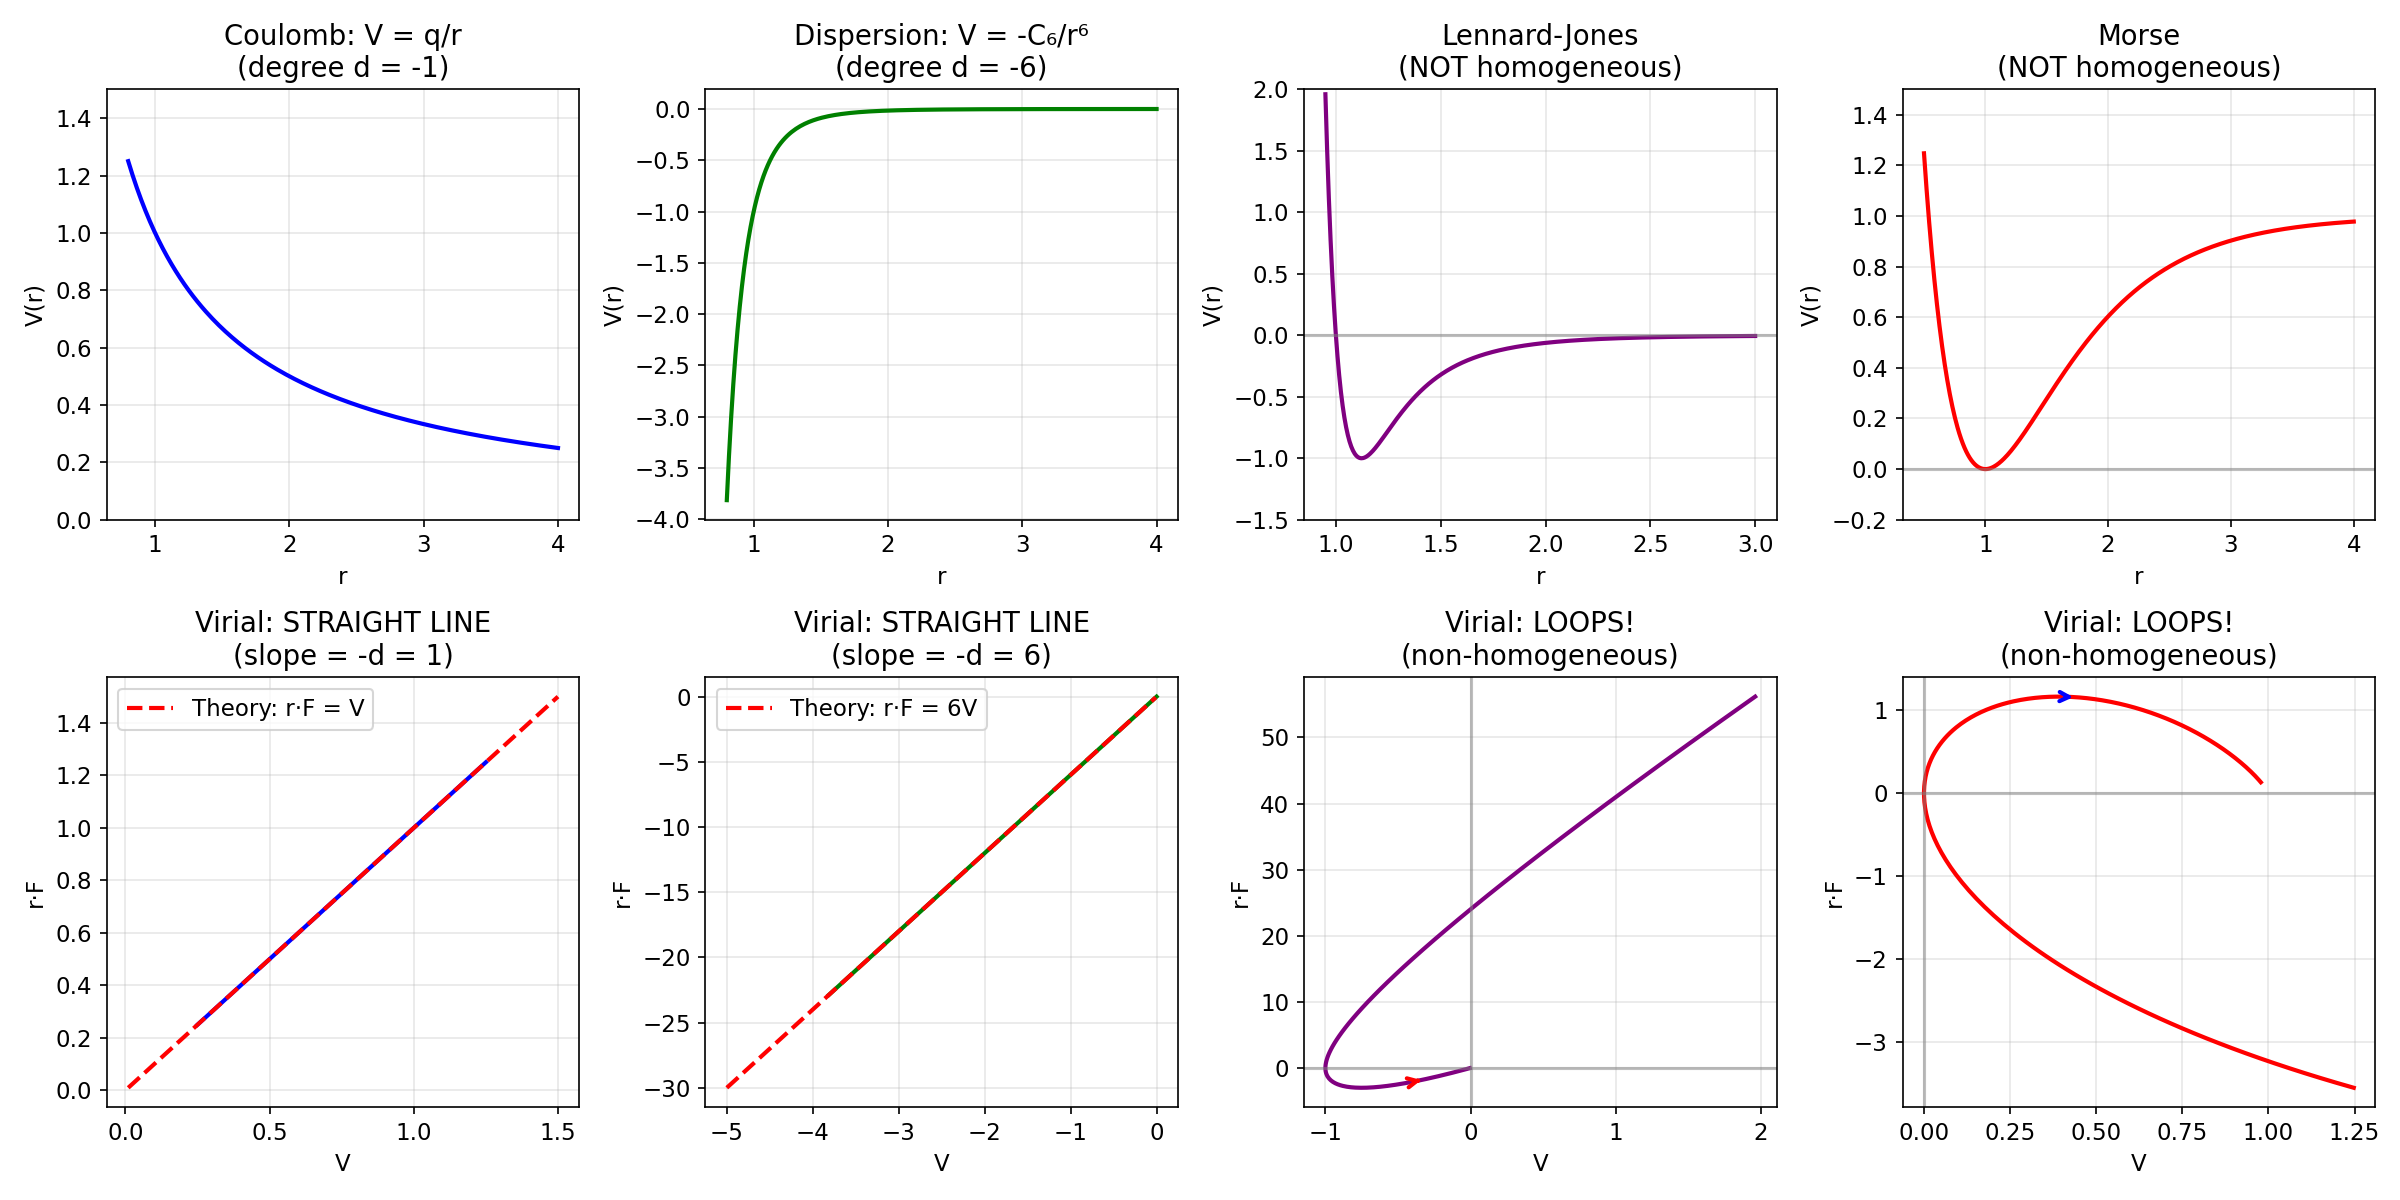
\includegraphics[width=\columnwidth]{figures/rose_uber/fig_virial_plots.png}
  \caption{Virial plots $rF(r)$ versus $V(r)$ for four pair potentials. (a,b)~Homogeneous potentials (Coulomb, dispersion) produce straight lines with slope $-d$. (c,d)~Non-homogeneous potentials (Morse, Lennard-Jones) form loops, indicating that no single power law describes the interaction at all separations.}
  \label{fig:virial}
\end{figure}

%-----------------------------------------------------------------------------
\subsection{Universal binding energy relations}
\label{sec:uber}
%-----------------------------------------------------------------------------

Rose, Smith, Guinea, and Ferrante~\cite{Rose1984,Ferrante1983} demonstrated that metallic and covalent binding energy curves collapse onto a universal form when expressed in scaled coordinates. The Rose equation of state (also called the universal binding energy relation, UBER) is
\begin{equation}
  E(a^*) = -E_c \bigl(1 + a^*\bigr) e^{-a^*},
  \label{eq:rose}
\end{equation}
where
\begin{equation}
  a^* = (r - r_e) / l
  \label{eq:astar}
\end{equation}
is the scaled interatomic distance. Here $E_c$ is the cohesive energy (well depth), $r_e$ is the equilibrium distance, and $l$ is a characteristic length scale related to the curvature at equilibrium~\cite{Vinet1987,Banerjea1988}.

An analogous universality exists for the Lennard-Jones potential: defining reduced variables $r^* = r/\sigma$ and $V^* = V/\varepsilon$, all LJ curves collapse to a single master curve $V^*(r^*) = 4[(r^*)^{-12} - (r^*)^{-6}]$. The parameters $(\varepsilon, \sigma)$ fully encode the material-specific information.

In both cases, diverse binding curves that appear qualitatively different collapse onto a \emph{single universal shape} when the material-specific scaling parameters are factored out (Fig.~\ref{fig:collapse}). This suggests that the scaling parameters, rather than the full energy curve, are the natural targets for machine learning.

\begin{figure*}[t]
  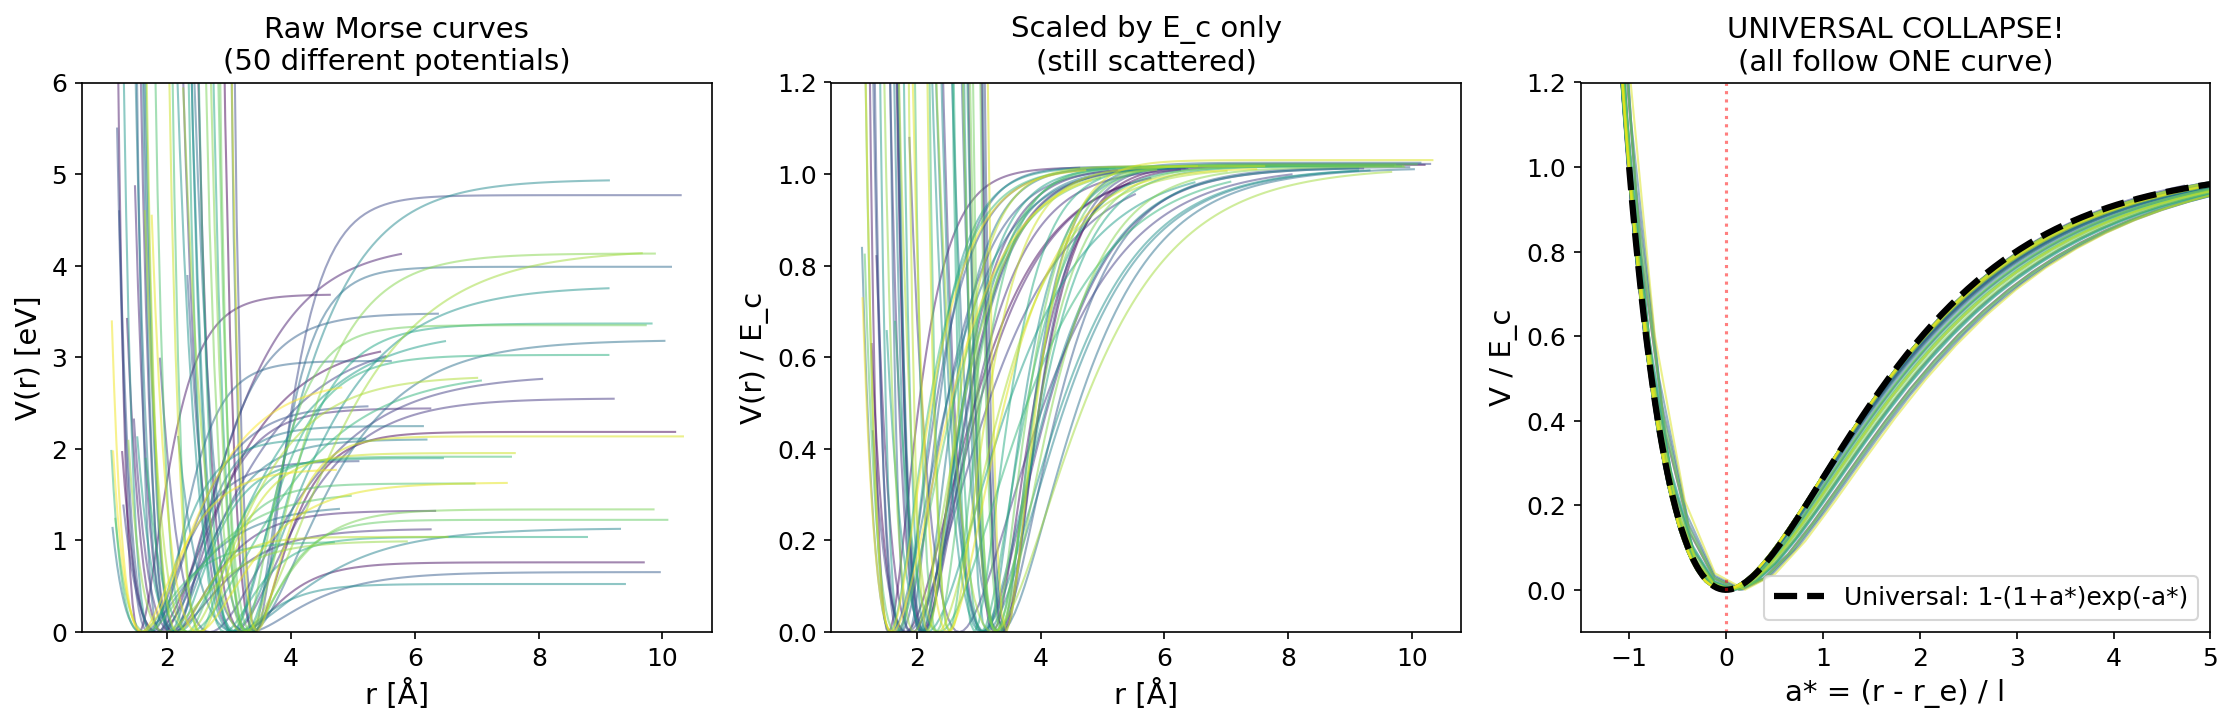
\includegraphics[width=0.48\textwidth]{figures/rose_uber/fig2_universal_collapse.png}%
  \hfill%
  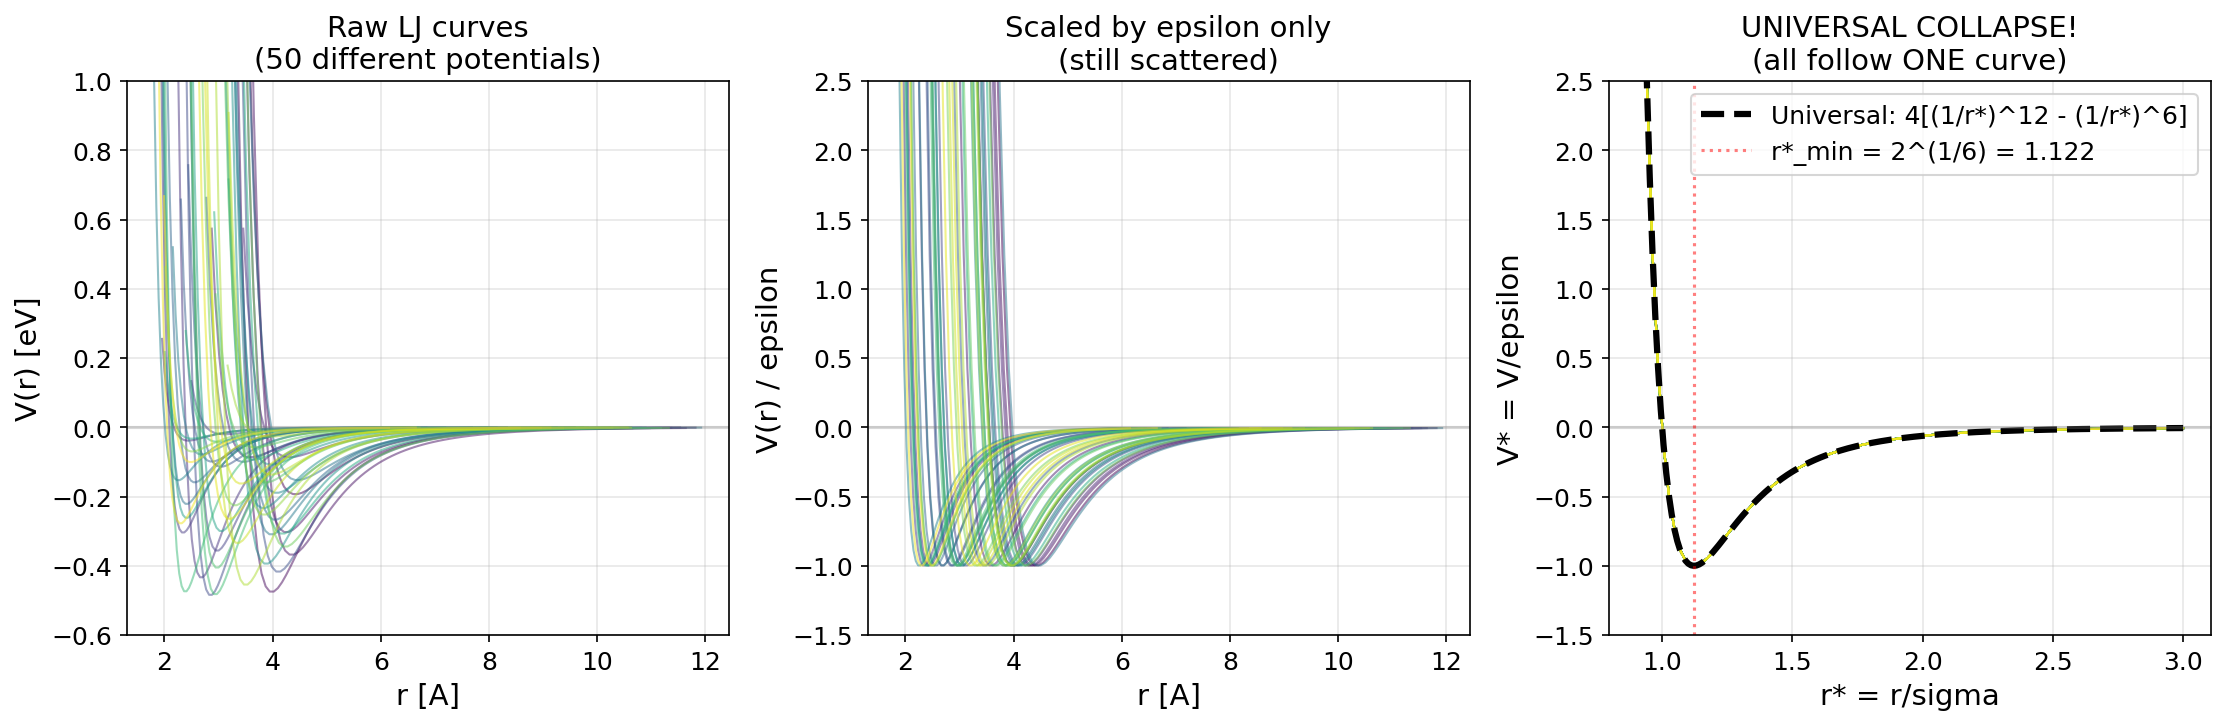
\includegraphics[width=0.48\textwidth]{figures/lennard_jones/fig2_lj_universal_collapse.png}
  \caption{Universal collapse of binding energy curves. Left (a--c): Morse potentials with diverse well depths and equilibrium distances collapse onto the universal Rose/UBER form $E/E_c$ versus $a^* = (r-r_e)/l$. Right (d--f): Lennard-Jones potentials collapse by construction onto $V/\varepsilon$ versus $r/\sigma$. The scaling parameters vary smoothly with descriptors, making them natural regression targets.}
  \label{fig:collapse}
\end{figure*}

%-----------------------------------------------------------------------------
\subsection{Adaptive parameter learning}
\label{sec:adaptive}
%-----------------------------------------------------------------------------

Motivated by the success of aPBE0~\cite{Khan2025}, we hypothesize that machine learning models can more efficiently learn interatomic potentials by predicting the universal scaling parameters as functions of atomic environment descriptors, rather than directly learning the energy surface $V(r)$.

The rationale is threefold:
\begin{enumerate}
  \item \textbf{Dimensionality reduction.} Two to three scalar parameters encode the essential physics of the binding curve, compared to $\sim$50 discretized energy values for the direct approach.
  \item \textbf{Bounded, smooth targets.} The scaling parameters have physical bounds and vary smoothly with atomic environment (Fig.~\ref{fig:collapse}), making them easier regression targets.
  \item \textbf{Physics-informed extrapolation.} Within physically meaningful parameter bounds, the analytical functional form guarantees correct qualitative behavior---short-range repulsion, a well-defined minimum, and long-range decay---even for configurations outside the training distribution. In practice, predicted parameters are clipped to physical ranges (e.g., $E_c > 0$, $r_e > 0$), which enforces these guarantees at the cost of introducing mild non-differentiability at the clipping boundaries.
  \item \textbf{Analytical derivatives.} Because the energy is expressed as a known function of $r$ and a few parameters, forces $F(r) = -dV/dr$ are obtained analytically. Unlike direct ML, which requires numerical differentiation or separate force-training networks, the adaptive approach guarantees smooth, conservative forces with correct asymptotics at no additional cost.
\end{enumerate}

The analogy to aPBE0 is direct:
\begin{center}
\begin{tabular}{lll}
  \toprule
  aPBE0 & Rose/UBER & Lennard-Jones \\
  \midrule
  $\mathbf{d} \to \alpha$ & $\mathbf{d} \to (E_c, r_e, l)$ & $\mathbf{d} \to (\varepsilon, \sigma)$ \\
  $E_\mathrm{xc}[\alpha]$ & $V[E_c, r_e, l]$ & $V[\varepsilon, \sigma]$ \\
  \bottomrule
\end{tabular}
\end{center}
In each case, a machine learning model predicts bounded, smooth parameters for a known physics equation, rather than learning the output quantity directly.


%=============================================================================
\section{Computational Methods}
\label{sec:methods}
%=============================================================================

%-----------------------------------------------------------------------------
\subsection{Model systems}
\label{sec:model_systems}
%-----------------------------------------------------------------------------

Two model potentials were studied to demonstrate the generality of the adaptive approach.

\textbf{Morse/Rose system.} Morse potentials [Eq.~\eqref{eq:morse}] served as ``ground truth'' binding curves, parameterized by well depth $D_e$, stiffness $a$, and equilibrium distance $r_e$. Rose parameters $(E_c, r_e^\mathrm{Rose}, l)$ were obtained for each Morse curve by nonlinear least-squares fitting of Eq.~\eqref{eq:rose} using the Levenberg--Marquardt algorithm (\textsc{SciPy} \texttt{curve\_fit}~\cite{Virtanen2020}), with bounds $E_c \in [0.01, 20]$~eV, $r_e \in [0.5, 10]$~\AA, and $l \in [0.01, 5]$~\AA.

\textbf{Lennard-Jones system.} LJ potentials [Eq.~\eqref{eq:lj}] served as a second test case where the scaling parameters $(\varepsilon, \sigma)$ are the \emph{native} parameters of the potential form, requiring no fitting step.

%-----------------------------------------------------------------------------
\subsection{Synthetic dataset generation}
\label{sec:datasets}
%-----------------------------------------------------------------------------

Descriptors $(d_1, d_2)$ served as proxies for local atomic environment features, analogous to SOAP~\cite{Bartok2010} or ACE~\cite{Drautz2019} descriptors in production MLIPs. Potential parameters were generated as linear functions of descriptors.

\textbf{Morse/Rose datasets.} Morse parameters were set as $D_e = 0.5 + 2.0\, d_1$~eV, $r_e = 1.5 + 0.5\, d_2$~\AA, and $a = 1.5$~\AA$^{-1}$ (fixed). Training descriptors were sampled uniformly: $d_1, d_2 \sim \mathcal{U}(0.5, 1.5)$, yielding $D_e \in [1.5, 3.5]$~eV. Extrapolation test data used $d_1 \sim \mathcal{U}(2.5, 4.0)$, yielding $D_e \in [5.5, 8.5]$~eV. Energy curves were evaluated on 50 points spanning $r \in [0.7\, r_e, 3.0\, r_e]$.

\textbf{Lennard-Jones datasets.} LJ parameters were set as $\sigma = 2.5 + 0.5\, d_1$~\AA\ and $\varepsilon = 0.05 + 0.1\, d_2$~eV. Training descriptors used $d_1, d_2 \sim \mathcal{U}(0.5, 1.5)$, yielding $\sigma \in [2.75, 3.25]$~\AA. Extrapolation test data used $d_1 \sim \mathcal{U}(2.5, 4.0)$, yielding $\sigma \in [3.75, 4.50]$~\AA.

Critically, all LJ energy curves were evaluated on a \emph{fixed} radial grid of 50 points spanning $r \in [2.5, 12.0]$~\AA, independent of $\sigma$. A $\sigma$-scaled grid (e.g., $r \in [0.9\sigma, 2.5\sigma]$) renders $\sigma/r$ constant across samples, reducing the descriptor-to-curve mapping to a trivial linear dependence on $\varepsilon$ alone. The fixed grid preserves the genuinely nonlinear dependence of $V(r)$ on $\sigma$ at fixed interatomic distances, which is the physically relevant scenario: in real simulations, atomic coordinates do not rescale with potential parameters.

%-----------------------------------------------------------------------------
\subsection{Machine learning models}
\label{sec:ml_models}
%-----------------------------------------------------------------------------

Two approaches were compared throughout. Both receive the same descriptor inputs $\mathbf{d} = (d_1, d_2)$; the only difference is the learning target. The descriptor-to-parameter relationships (e.g., $\sigma = 2.5 + 0.5\, d_1$) are unknown to the ML model and must be learned from training examples.

\textbf{Direct learning.} A Ridge regression model maps descriptors directly to the discretized potential energy curve:
\begin{equation}
  \mathbf{d} = (d_1, d_2) \;\xrightarrow{\text{Ridge}}\; \{V(r_i)\}_{i=1}^{N_r}.
  \label{eq:direct}
\end{equation}

\textbf{Adaptive learning.} A Ridge regression model maps descriptors to the universal scaling parameters, which are then transformed to energies via the analytical physics equation:
\begin{equation}
  \mathbf{d} \;\xrightarrow{\text{Ridge}}\; \boldsymbol{\theta} \;\xrightarrow{\text{physics}}\; V_{\boldsymbol{\theta}}(r),
  \label{eq:adaptive}
\end{equation}
where $\boldsymbol{\theta} = (E_c, r_e, l)$ for Rose/UBER or $\boldsymbol{\theta} = (\varepsilon, \sigma)$ for LJ. Predicted parameters were clipped to physically meaningful ranges (e.g., $E_c > 0.01$~eV, $r_e > 0.5$~\AA, $l > 0.01$~\AA) before curve reconstruction. In practice, clipping was rarely triggered: for the extrapolation test sets, fewer than 1\% of predicted parameters fell outside the physical bounds.

Ridge regression with regularization parameter $\alpha = 1.0$ was employed for both approaches. All input features and output targets were standardized (zero mean, unit variance) prior to training using \texttt{StandardScaler}~\cite{Pedregosa2011}. The scaler was fit on training data only and applied to test data.

Ridge regression (a global linear model) was chosen deliberately over kernel ridge regression (KRR) with radial basis function (RBF) kernels. While KRR can capture nonlinear relationships within the training domain, the RBF kernel $K(\mathbf{x}, \mathbf{x}') = \exp(-\gamma\|\mathbf{x} - \mathbf{x}'\|^2)$ decays to zero for test points far from training data, causing predictions to regress toward the training mean in extrapolative regimes. Ridge regression, as a global linear model, can extrapolate linearly---providing a controlled baseline that isolates the structural advantage of the adaptive approach without confounding kernel effects. We verified this choice empirically: KRR with optimized hyperparameters yielded identical performance for both direct and adaptive approaches in the extrapolation regime, with no improvement as training set size increased (see Supplemental Material).

%-----------------------------------------------------------------------------
\subsection{Evaluation metrics and protocols}
\label{sec:evaluation}
%-----------------------------------------------------------------------------

Model performance was assessed using the mean absolute error (MAE),
\begin{equation}
  \mathrm{MAE} = \frac{1}{N_\mathrm{test} N_r} \sum_{j=1}^{N_\mathrm{test}} \sum_{i=1}^{N_r} |V_j(r_i)^\mathrm{true} - V_j(r_i)^\mathrm{pred}|,
\end{equation}
and the coefficient of determination ($R^2$),
\begin{equation}
  R^2 = 1 - \frac{\sum_{j,i}(V_{j,i}^\mathrm{true} - V_{j,i}^\mathrm{pred})^2}{\sum_{j,i}(V_{j,i}^\mathrm{true} - \bar{V}^\mathrm{true})^2},
\end{equation}
computed over all test curves and grid points jointly.

Four systematic experiments were conducted for each model system:

\textbf{Experiment 1: Data efficiency.} Training set sizes $N \in \{10, 15, 20, \ldots, 160\}$ were evaluated against a fixed test set of 50 samples in the extrapolation regime. Five independent random seeds per training size were used for learning curve computations.

\textbf{Experiment 2: Interpolation versus extrapolation.} A fixed training set ($N = 100$) was evaluated against five test regimes of increasing extrapolation severity, from interpolation ($d_1 \in [1.3, 2.2]$) to strong extrapolation ($d_1 \in [3.5, 4.5]$).

\textbf{Experiment 3: Noise robustness.} Gaussian noise with amplitude $\sigma_\mathrm{noise} \in \{0, 1, 2, 5, 10, 15, 20\}\%$ of the mean $|V|$ was added to training energy curves. Test data remained noise-free.

\textbf{Experiment 4: Parameter interpretability.} The quality of predicted scaling parameters was assessed individually by computing $R^2$ and MAE between true and predicted parameter values in the extrapolation regime.

%-----------------------------------------------------------------------------
\subsection{DFT diatomics validation}
\label{sec:dft_methods}
%-----------------------------------------------------------------------------

To validate the adaptive approach on real quantum-chemical data, binding energy curves were computed for 30 homonuclear and heteronuclear diatomic molecules spanning the first three rows of the periodic table: H$_2$, LiH, BeH, BH, CH, NH, OH, HF, NaH, MgH, AlH, SiH, PH, SH, HCl, KH, Li$_2$, N$_2$, O$_2$, F$_2$, Na$_2$, Cl$_2$, LiF, NaF, NaCl, CO, NO, CN, BF, and AlF.

\textbf{Electronic structure.} All calculations used unrestricted Kohn--Sham DFT (UKS) with the PBE exchange-correlation functional~\cite{Perdew1996} and def2-SVP basis set~\cite{Weigend2005}, as implemented in PySCF~\cite{Sun2018}. UKS was used for all molecules, including closed-shell singlets, because restricted KS fails to describe spin-symmetry breaking at stretched geometries, causing SCF divergence for molecules such as F$_2$, Cl$_2$, and NaF. A three-level convergence strategy was employed: (i) UKS with 0.5 damping, (ii) UKS without damping, and (iii) UKS with Fermi smearing ($\sigma_\mathrm{el} = 0.01$~Ha). All 30 molecules converged successfully.

\textbf{Binding curves.} For each molecule, 25 interatomic distances were sampled uniformly from $0.7\, r_\mathrm{eq}$ to $5.0\, r_\mathrm{eq}$, where $r_\mathrm{eq}$ is the experimental equilibrium distance. Binding energies were computed as $E_\mathrm{bind}(r) = E_\mathrm{mol}(r) - E_{\mathrm{atom}_1} - E_{\mathrm{atom}_2}$, where atomic reference energies were obtained from spin-polarized UKS calculations in the correct ground-state spin multiplicity for each atom (e.g., doublet for H, triplet for O, quartet for N). Rose/UBER parameters $(E_c, r_e, l)$ were obtained by nonlinear least-squares fitting. Two molecules were excluded from the ML comparison due to high Rose fit residuals: H$_2$ (RMSE = 1.12~eV, UKS symmetry-breaking artifacts) and N$_2$ (RMSE = 2.09~eV, multi-reference character).

\textbf{Descriptors.} Fourteen atomic pair features were constructed for each molecule: atomic number ($Z_1$, $Z_2$), Pauling electronegativity ($\mathrm{EN}_1$, $\mathrm{EN}_2$), covalent radius ($r_{\mathrm{cov},1}$, $r_{\mathrm{cov},2}$), and first ionization energy ($\mathrm{IE}_1$, $\mathrm{IE}_2$), along with pairwise sums and differences of EN, $r_\mathrm{cov}$, and IE.

\textbf{Common grid.} Because different molecules have vastly different equilibrium distances (H$_2$: 0.74~\AA\ versus Na$_2$: 3.08~\AA), a common radial grid in raw coordinates would have negligible overlap. Instead, scaled coordinates $r_s = r / r_{\mathrm{cov,sum}}$ were used, where $r_{\mathrm{cov,sum}} = r_{\mathrm{cov},1} + r_{\mathrm{cov},2}$ is the sum of covalent radii (available from the descriptors, not from adaptive parameters). This yields a scaled overlap width of 3.11, covering the full binding well for all molecules. Importantly, the scaling uses only tabulated covalent radii (included in the descriptor set), not fitted parameters, so both direct and adaptive approaches operate on identical input grids.

\textbf{Cross-validation.} Two protocols were used:
\begin{itemize}
  \item \emph{Leave-one-out (LOO):} Each of the 28 molecules is held out once; the model trains on the remaining 27 and predicts the held-out curve. This tests interpolation.
  \item \emph{Leave-group-out (LGO):} Molecules are split by periodic table row. Training uses 15 molecules composed exclusively of row 1--2 atoms (H through Ne). Testing uses 13 molecules containing at least one row 3+ atom (Na through K). This tests extrapolation to heavier elements.
\end{itemize}


%=============================================================================
\section{Results}
\label{sec:results}
%=============================================================================

%-----------------------------------------------------------------------------
\subsection{Universal collapse and parameter smoothness}
\label{sec:collapse}
%-----------------------------------------------------------------------------

Figure~\ref{fig:collapse} demonstrates the universality underlying the adaptive approach. For the Rose/UBER system [Fig.~\ref{fig:collapse}(a--c)], Morse potentials with diverse well depths ($D_e = 1.5$--$3.5$~eV) and equilibrium distances ($r_e = 1.75$--$2.0$~\AA) collapse onto a single universal curve when expressed in scaled coordinates $E/E_c$ versus $a^* = (r - r_e)/l$. The scaling parameters vary smoothly and approximately linearly with the descriptor $d_1$ [Fig.~\ref{fig:collapse}(c)], making them ideal regression targets.

For the Lennard-Jones system [Fig.~\ref{fig:collapse}(d--f)], the collapse is exact by construction: $V/\varepsilon$ versus $r/\sigma$ gives a single master curve. The parameters $\sigma$ and $\varepsilon$ again vary linearly with descriptors [Fig.~\ref{fig:collapse}(f)].

This universality---diverse curves differing only in a few smooth, bounded parameters---is precisely what makes the adaptive approach effective. A model that learns these parameters inherits the correct functional form for free, while a model that learns $V(r)$ directly must rediscover the universal shape from data at each new configuration.

%-----------------------------------------------------------------------------
\subsection{Extrapolation performance}
\label{sec:extrapolation}
%-----------------------------------------------------------------------------

\begin{figure}[t]
  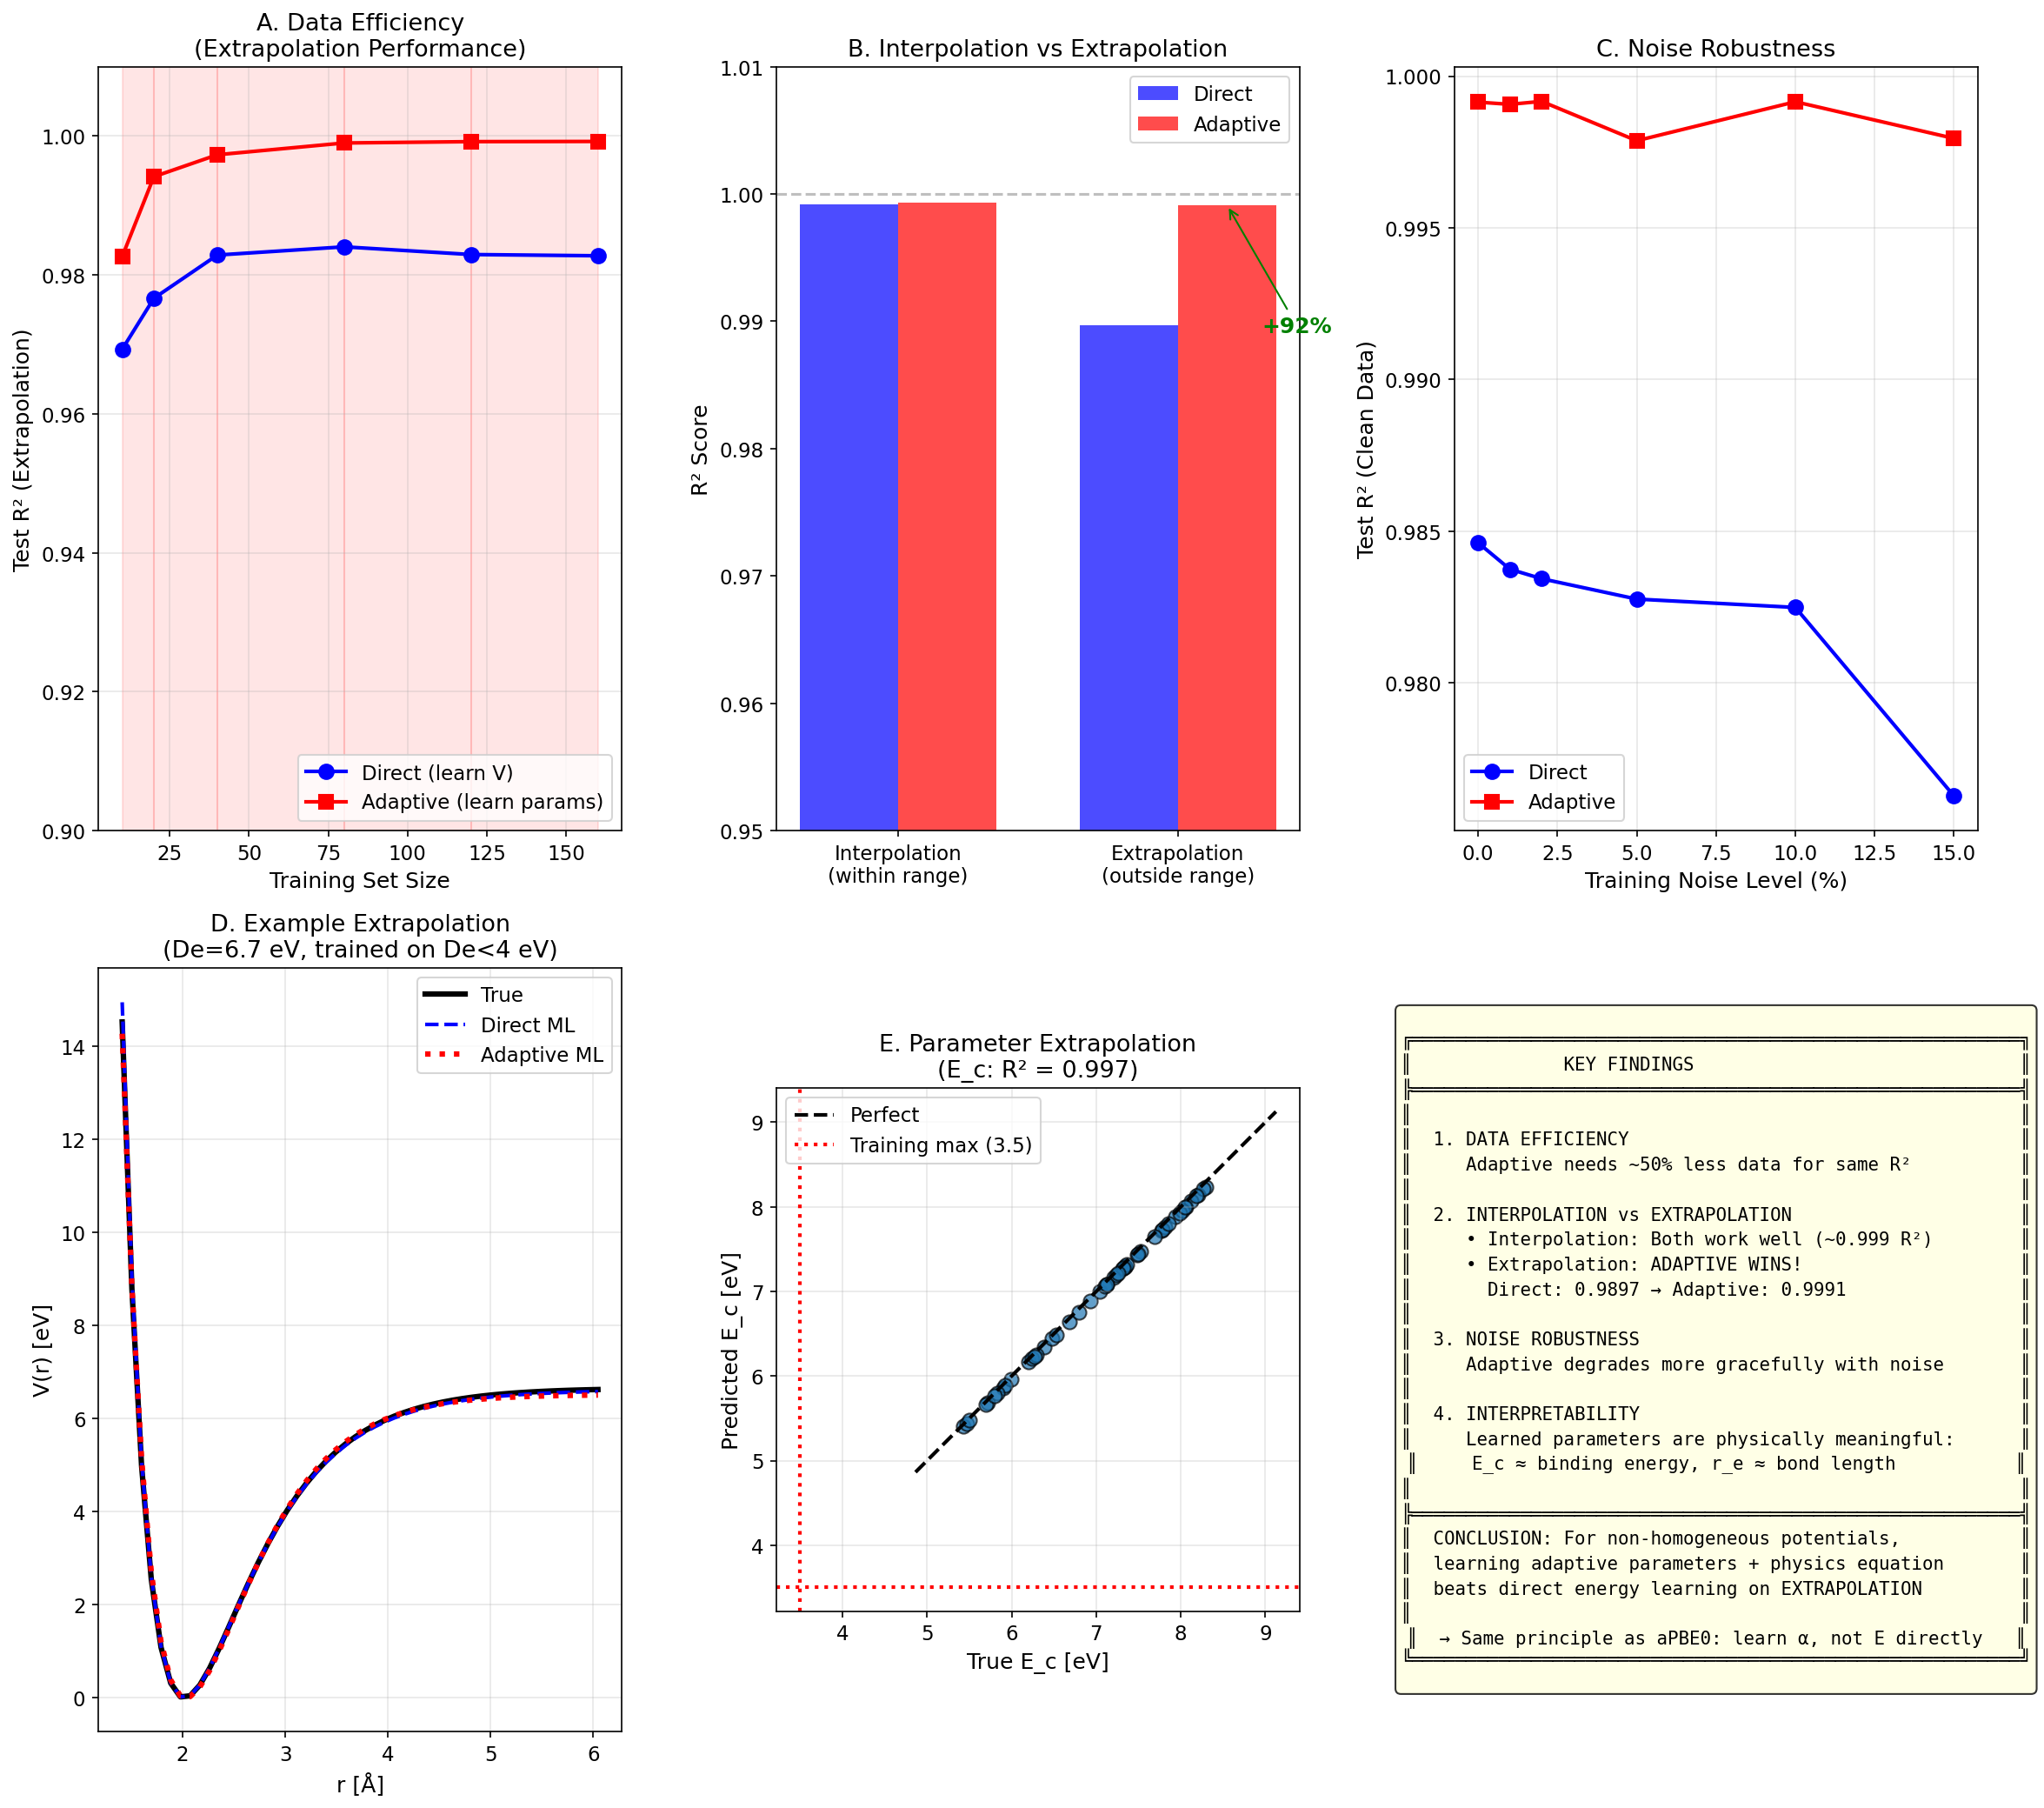
\includegraphics[width=\columnwidth]{figures/rose_uber/fig_refined_ml_demo.png}
  \caption{Rose/UBER system: comprehensive ML comparison. (a)~Data efficiency showing $R^2$ versus training set size. (b)~$R^2$ across interpolation and extrapolation test regimes. (c)~Noise robustness. (d)~Example extrapolation prediction. (e)~Parameter prediction quality (extrapolation). See text for details.}
  \label{fig:rose_results}
\end{figure}

\begin{figure}[t]
  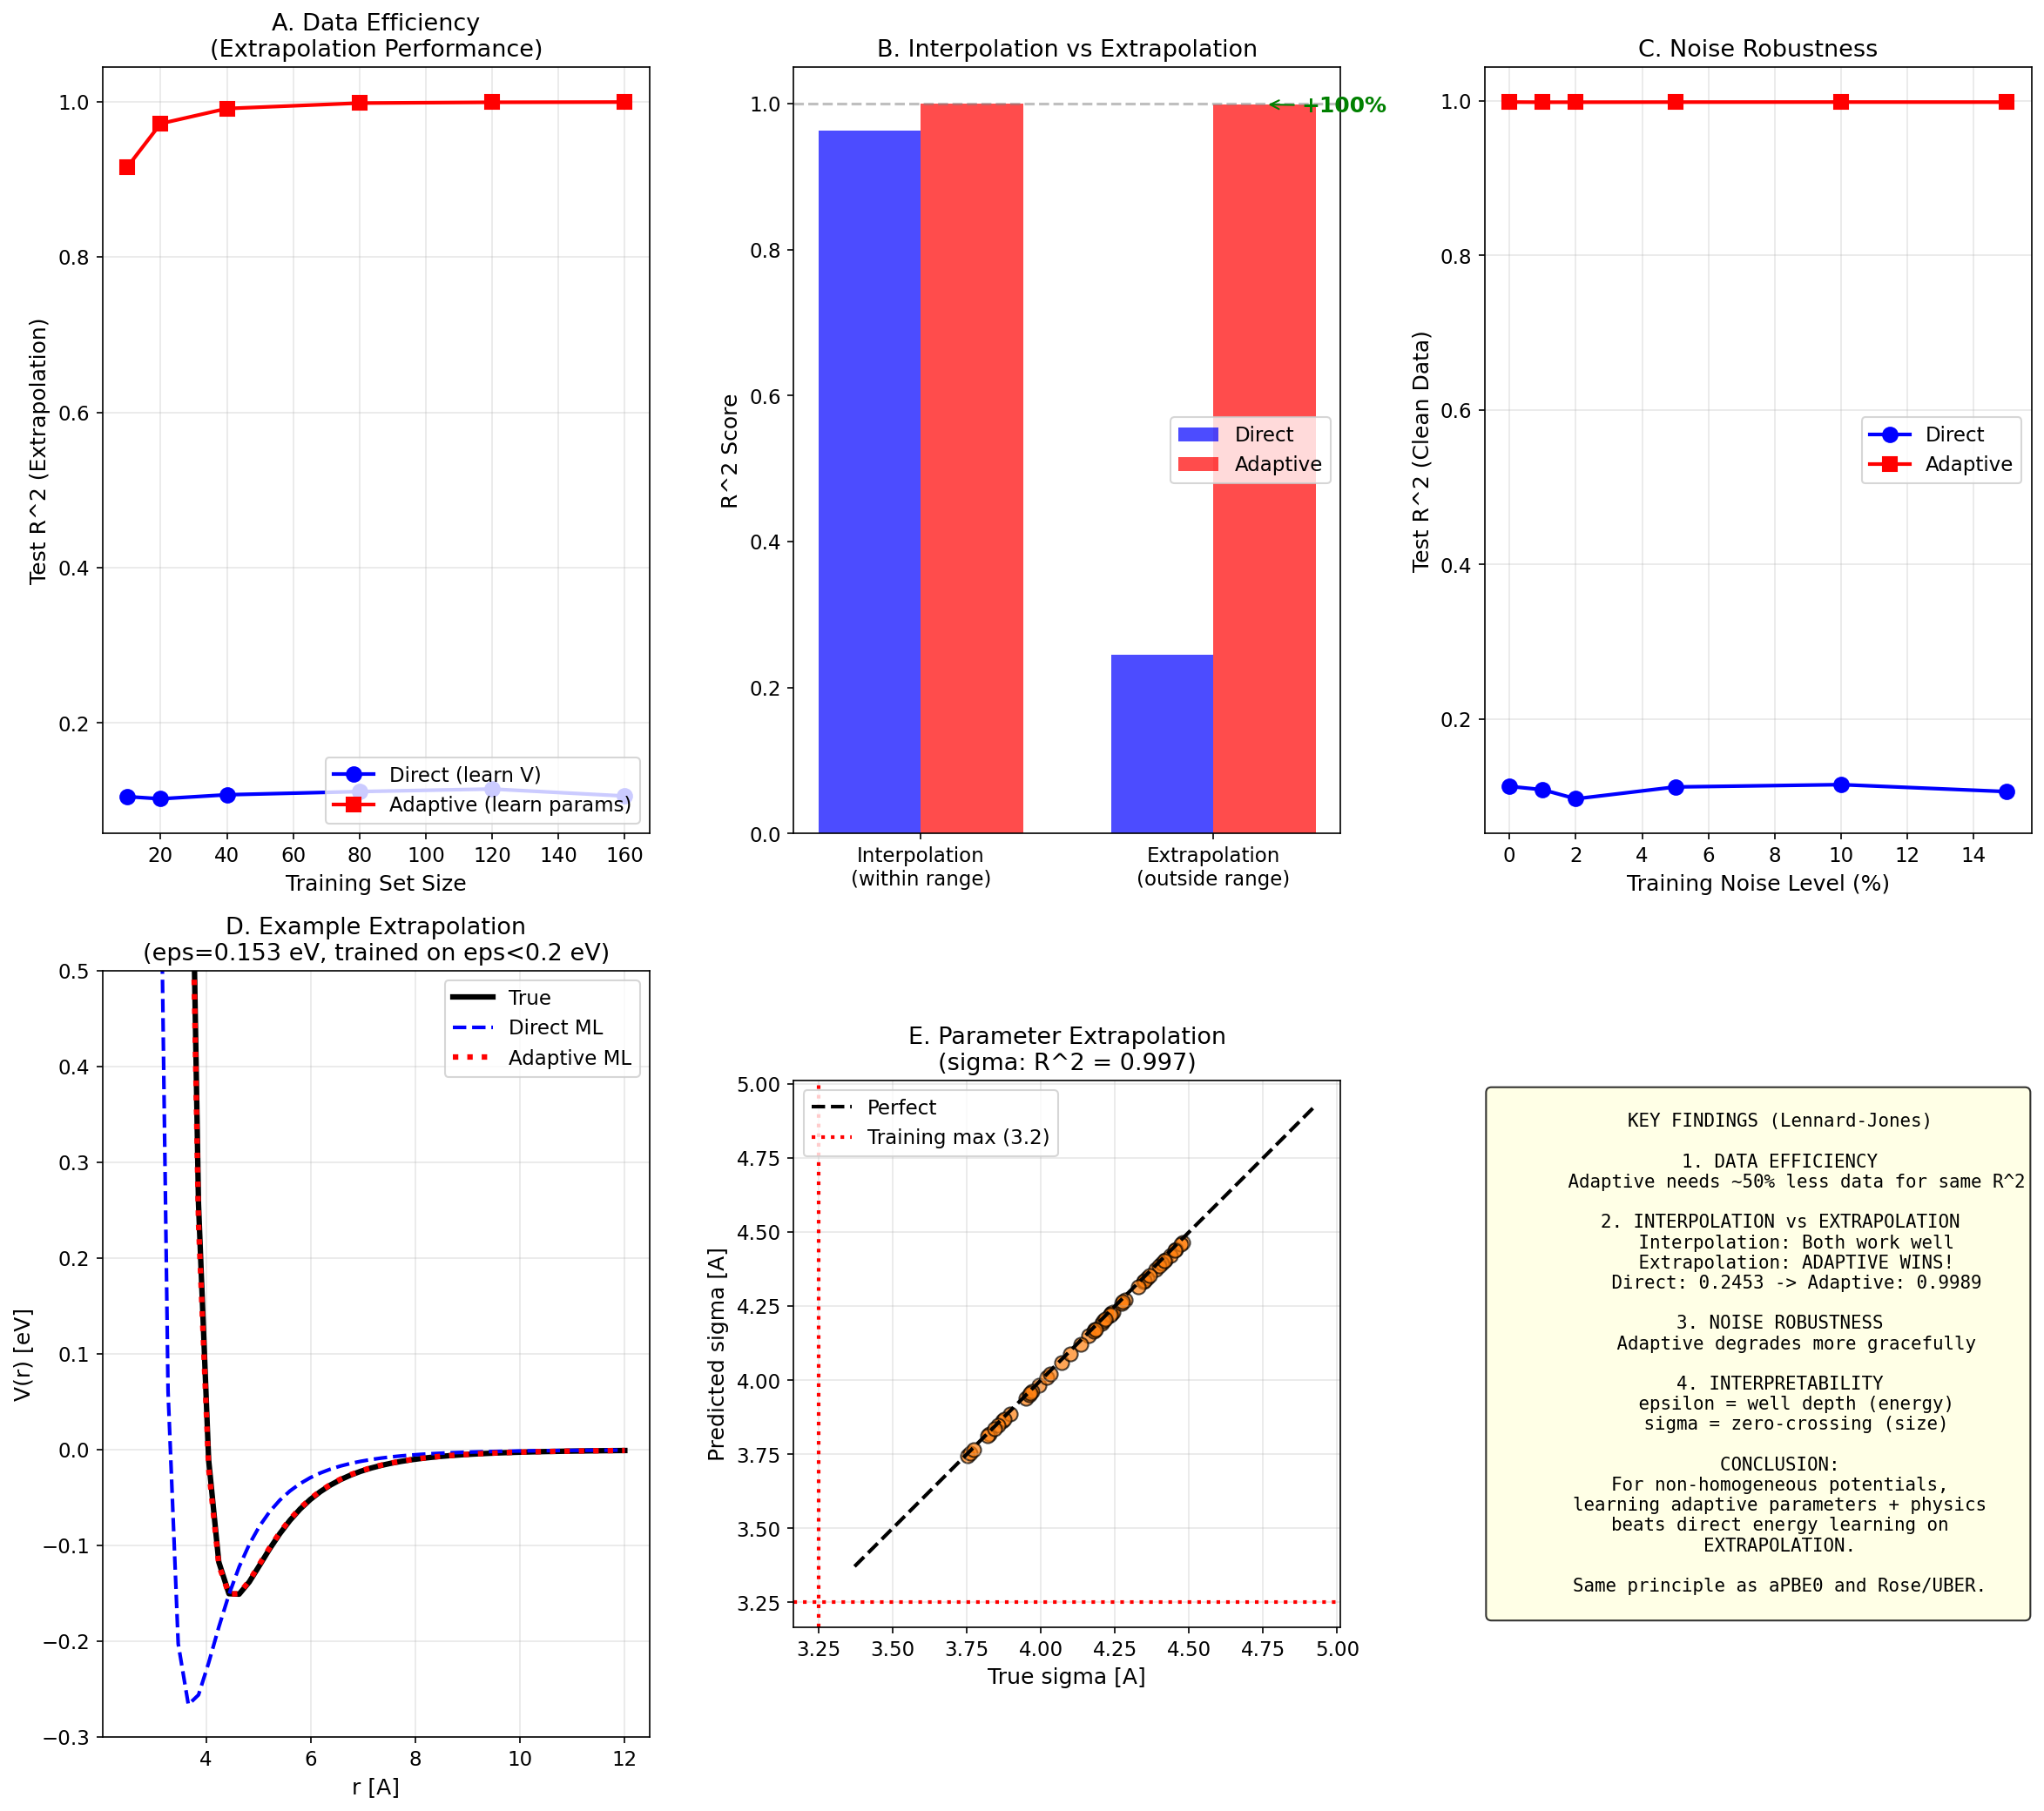
\includegraphics[width=\columnwidth]{figures/lennard_jones/fig_lj_refined_ml_demo.png}
  \caption{Lennard-Jones system: comprehensive ML comparison, same format as Fig.~\ref{fig:rose_results}. The dramatic failure of direct learning (gray) on the fixed grid reflects the nonlinear $\sigma$ dependence that a linear model cannot capture, while the adaptive approach (blue) circumvents this by learning $(\varepsilon, \sigma)$ directly.}
  \label{fig:lj_results}
\end{figure}

Figure~\ref{fig:rose_results}(d) shows a representative extrapolation example for the Rose/UBER system: the adaptive prediction (blue) closely tracks the true curve (black dashed), while the direct prediction (gray) systematically underestimates the well depth. Figure~\ref{fig:lj_results}(d) shows the corresponding LJ example, where the direct approach fails catastrophically---the predicted curve bears little resemblance to the true potential.

The learning curves (Fig.~\ref{fig:learning_curves}) provide the central quantitative comparison. For the Rose/UBER system [Fig.~\ref{fig:learning_curves}(a)], the extrapolation MAE follows power-law decay for both approaches, but with different exponents: $\mathrm{MAE}_\mathrm{adaptive} \propto N^{-0.57}$ versus $\mathrm{MAE}_\mathrm{direct} \propto N^{-0.30}$. At $N = 160$ training samples, the adaptive approach achieves $\mathrm{MAE} = 0.063 \pm 0.001$~eV compared to $0.144 \pm 0.016$~eV for direct learning---a $2.3\times$ improvement. The crossover occurs at approximately $N = 20$; below this, both approaches are comparable (Table~\ref{tab:learning_curves}).

For the Lennard-Jones system [Fig.~\ref{fig:learning_curves}(b)], the contrast is far more dramatic. The direct approach shows essentially no learning: $\mathrm{MAE}_\mathrm{direct} \propto N^{-0.03}$, remaining at $\sim$8--9~eV regardless of training set size. The adaptive approach, by contrast, achieves rapid decay: $\mathrm{MAE}_\mathrm{adaptive} \propto N^{-0.94}$, reaching $0.22 \pm 0.01$~eV at $N = 160$. This $42\times$ advantage partly reflects a function-class mismatch: the LJ potential at fixed $r$ depends nonlinearly on $\sigma$ through $(\sigma/r)^{12}$ and $(\sigma/r)^{6}$, which a linear model cannot represent. The adaptive approach sidesteps this by learning $\sigma$ as a linear function of descriptors and delegating the nonlinear transformation to the physics equation. However, even nonlinear direct baselines (polynomial features up to degree 6) fail to match the adaptive approach for extrapolation (Sec.~\ref{sec:capacity}), confirming that the advantage is not merely linear versus nonlinear but reflects the correct functional form.

\begin{figure*}[t]
  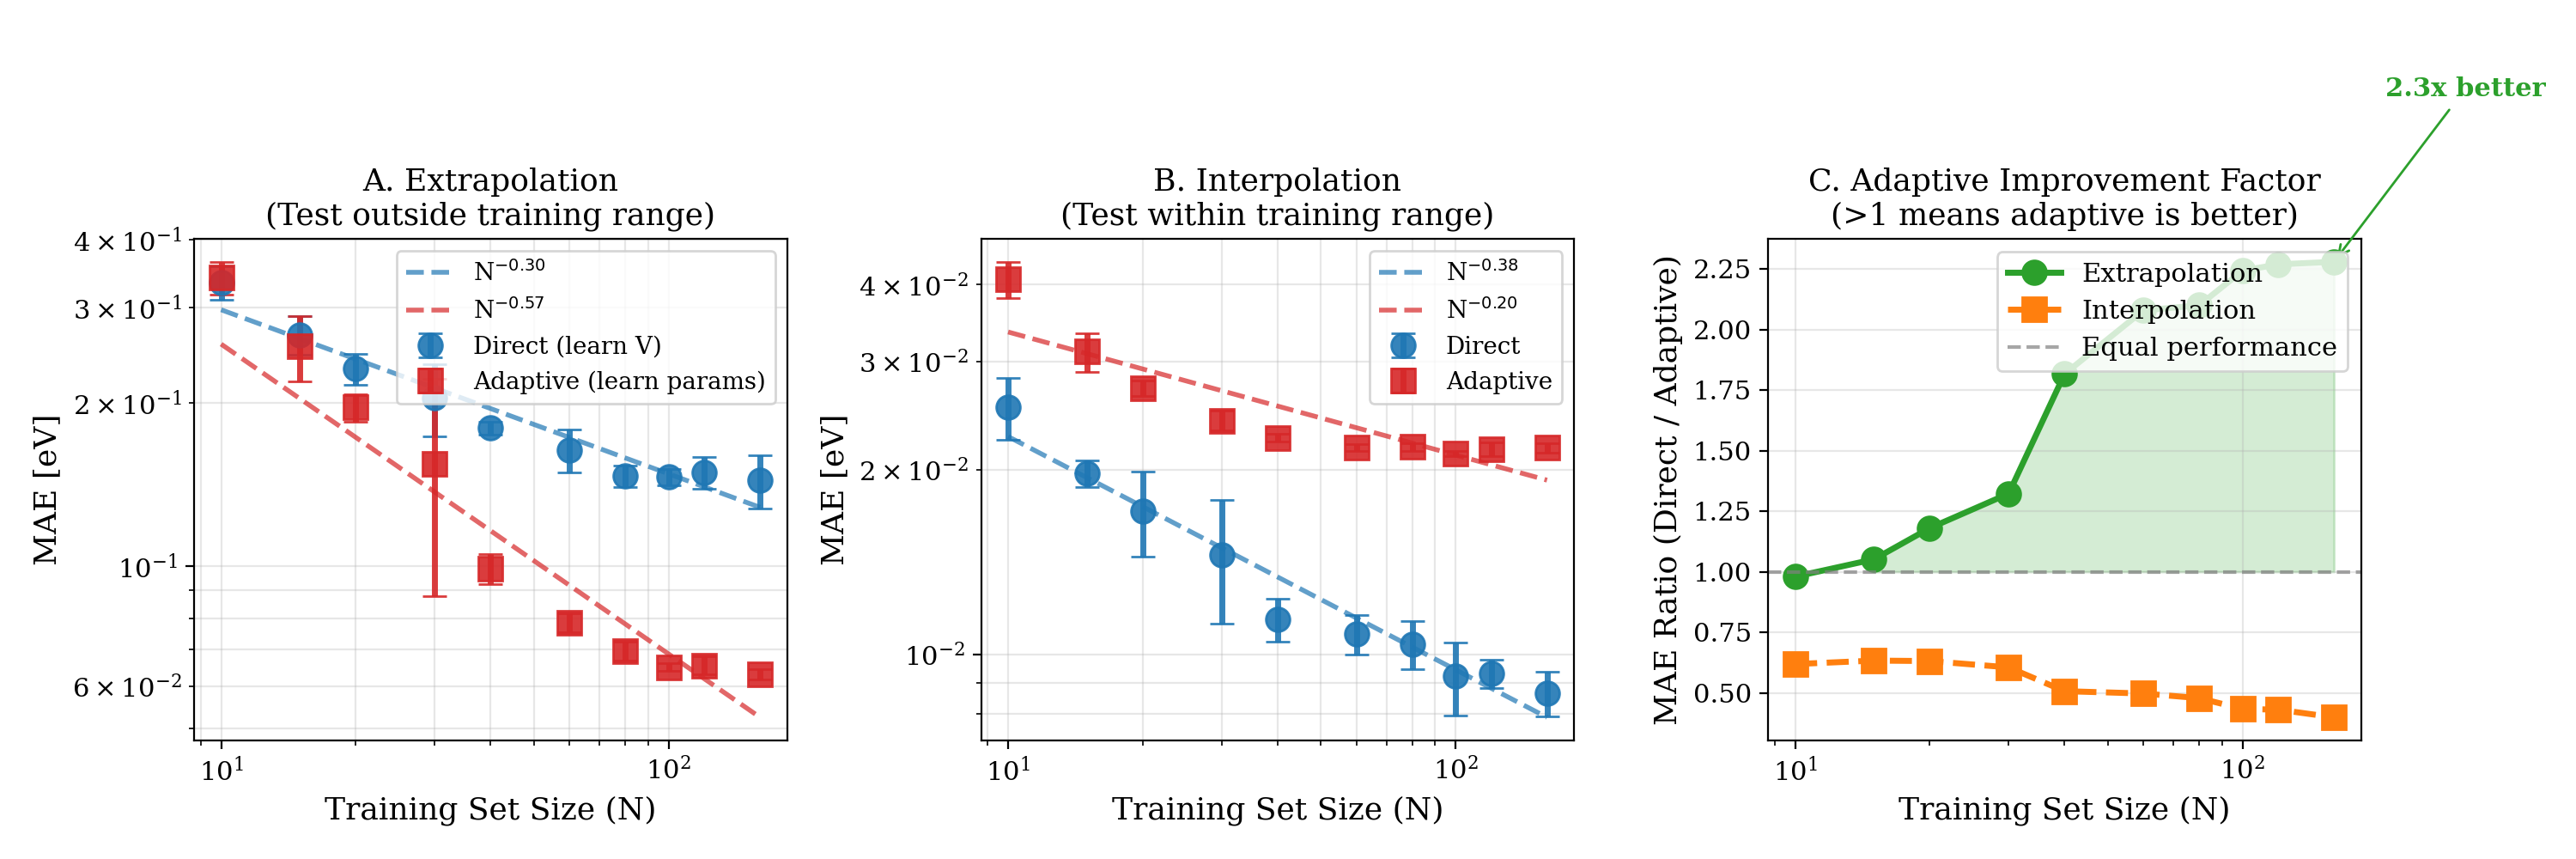
\includegraphics[width=0.48\textwidth]{figures/rose_uber/fig_learning_curves_combined.png}%
  \hfill%
  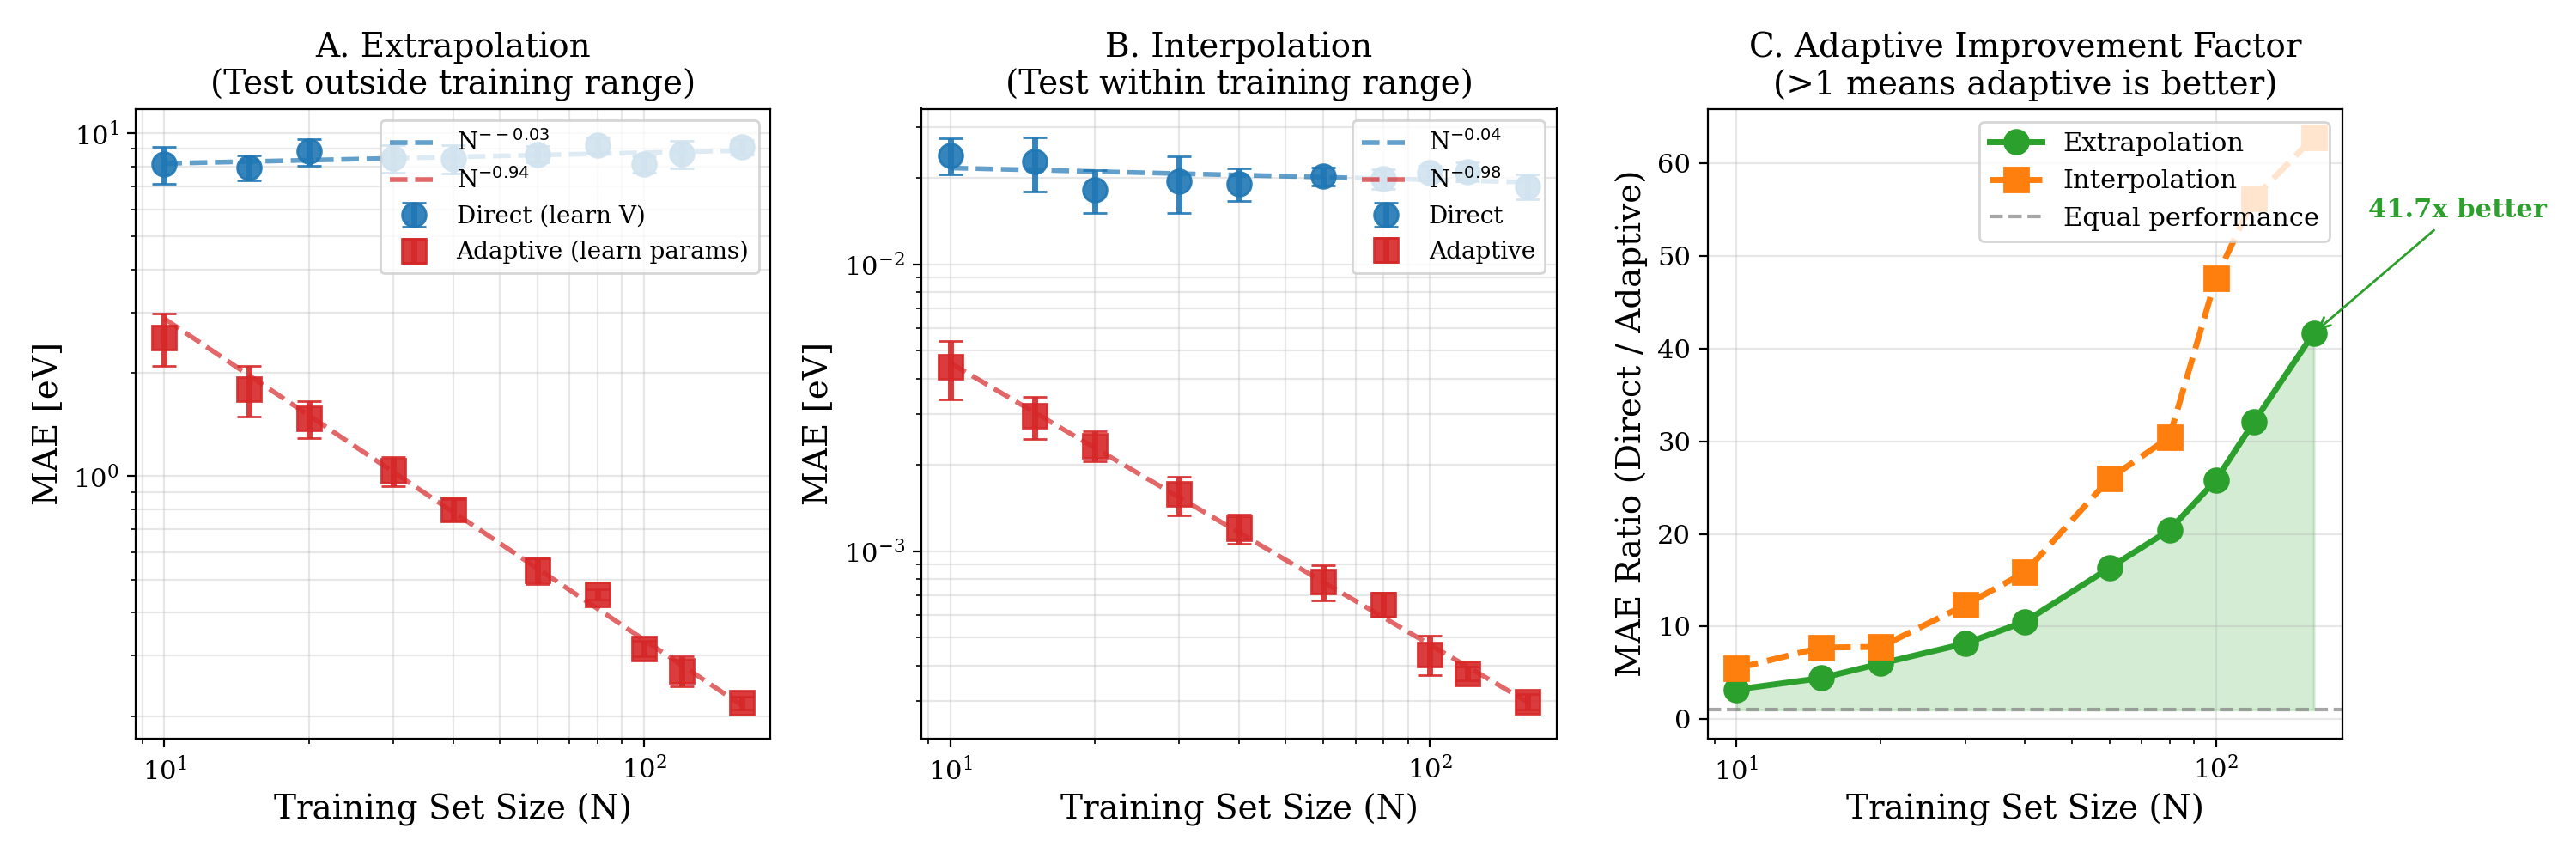
\includegraphics[width=0.48\textwidth]{figures/lennard_jones/fig_lj_learning_curves_combined.png}
  \caption{Learning curves for the Rose/UBER system (left panels) and Lennard-Jones system (right panels). For each: extrapolation MAE versus training set size with power-law fits, interpolation MAE, and ratio of direct to adaptive MAE (values $>1$ indicate adaptive advantage). Shaded regions indicate $\pm 1$ standard deviation over 5 random seeds. The dashed lines show power-law fits $\mathrm{MAE} \propto N^{-\beta}$ with exponents $\beta$ as indicated.}
  \label{fig:learning_curves}
\end{figure*}

\begin{table}[t]
  \caption{Learning curve power-law exponents $\beta$ (MAE $\propto N^{-\beta}$) and MAE ratio at $N = 160$ training samples, averaged over 5 random seeds. Higher $\beta$ indicates faster learning; ratio $> 1$ favors the adaptive approach.}
  \label{tab:learning_curves}
  \begin{ruledtabular}
  \begin{tabular}{llccc}
    System & Regime & $\beta_\mathrm{direct}$ & $\beta_\mathrm{adaptive}$ & Ratio ($N\!=\!160$) \\
    \hline
    Rose/UBER & Extrapolation & $0.30$ & $0.57$ & $2.3\times$ \\
    Rose/UBER & Interpolation & $0.38$ & $0.20$ & $0.40\times$ \\
    LJ & Extrapolation & $0.03$ & $0.94$ & $42\times$ \\
    LJ & Interpolation & $0.04$ & $0.98$ & $63\times$ \\
  \end{tabular}
  \end{ruledtabular}
\end{table}

Notably, the adaptive approach also dominates for LJ \emph{interpolation} ($63\times$ advantage at $N = 160$), because the nonlinear $\sigma$ dependence at fixed grid points is difficult for Ridge regression even within the training range. For Rose/UBER interpolation, however, direct learning wins ($0.40\times$, i.e., direct is $2.5\times$ better). This is because the Rose equation is an \emph{approximation} to the Morse potential---the fitting step introduces a systematic residual of $\sim$0.02~eV that sets a floor on the adaptive approach's accuracy. When the physics equation is exact (as for LJ), no such floor exists.

%-----------------------------------------------------------------------------
\subsection{Extrapolation severity and noise robustness}
\label{sec:severity_noise}
%-----------------------------------------------------------------------------

Figure~\ref{fig:rose_results}(b) and \ref{fig:lj_results}(b) show how $R^2$ degrades as the test set moves further from the training distribution. For the Rose/UBER system, the adaptive approach maintains $R^2 > 0.999$ even at strong extrapolation ($d_1 \in [3.5, 4.5]$, well beyond the training range of $[0.5, 1.5]$), while the direct approach drops to $R^2 = 0.988$. For LJ, the direct approach degrades from $R^2 = 0.93$ (interpolation) to $R^2 = 0.21$ (strong extrapolation), while the adaptive approach remains at $R^2 > 0.998$ throughout (Table~\ref{tab:summary}).

Both approaches show robustness to training noise [Fig.~\ref{fig:rose_results}(c) and \ref{fig:lj_results}(c)]. For Rose/UBER, the adaptive approach maintains $R^2 > 0.99$ up to 15\% noise, degrading to $R^2 = 0.984$ at 20\% noise; the direct approach degrades more steadily from $R^2 = 0.982$ to $0.973$. For LJ, the adaptive approach is essentially unaffected by noise ($R^2 > 0.998$ at all noise levels), while the direct approach remains at $R^2 \approx 0.10$ regardless---already failing in the absence of noise.

The noise robustness of the adaptive approach follows from the dimensionality reduction: fitting two to three parameters from a noisy energy curve effectively averages out the noise, while predicting 50 individual energy values amplifies it.

%-----------------------------------------------------------------------------
\subsection{Parameter interpretability}
\label{sec:params}
%-----------------------------------------------------------------------------

Figures~\ref{fig:rose_results}(e) and \ref{fig:lj_results}(e) show parity plots for the predicted versus true scaling parameters in the extrapolation regime. For the Rose/UBER system: $R^2(E_c) = 0.998$, $R^2(r_e) = 1.000$, $R^2(l) = 0.986$. For LJ: $R^2(\varepsilon) = 1.000$ (MAE = 0.0003~eV), $R^2(\sigma) = 0.998$ (MAE = 0.011~\AA). The parameters extrapolate correctly well beyond the training range, confirming that the smooth, bounded nature of these targets facilitates generalization.

These predicted parameters have direct physical meaning: $E_c$ tracks the binding energy, $r_e$ the bond length, and $l$ the stiffness. This interpretability is a ``free'' benefit of the adaptive approach---a direct model provides no analogous physical insight.

%-----------------------------------------------------------------------------
\subsection{Force prediction}
\label{sec:forces}
%-----------------------------------------------------------------------------

A practical advantage of the adaptive approach is that analytical derivatives $dV/dr$ are obtained for free. Given predicted parameters $(\varepsilon, \sigma)$, the LJ gradient at any interatomic distance is
\begin{equation}
  \frac{dV}{dr} = \frac{24\varepsilon}{r}\left[\left(\frac{\sigma}{r}\right)^6 - 2\left(\frac{\sigma}{r}\right)^{12}\right],
  \label{eq:lj_force}
\end{equation}
which is exact, grid-independent, and continuous. For Rose/UBER:
\begin{equation}
  \frac{dV}{dr} = \frac{E_c\, a^*}{l}\, e^{-a^*}.
  \label{eq:rose_force}
\end{equation}
Direct learning, by contrast, requires numerical differentiation of the discretized energy curve, introducing both discretization error and amplified prediction noise.

\begin{figure}[t]
  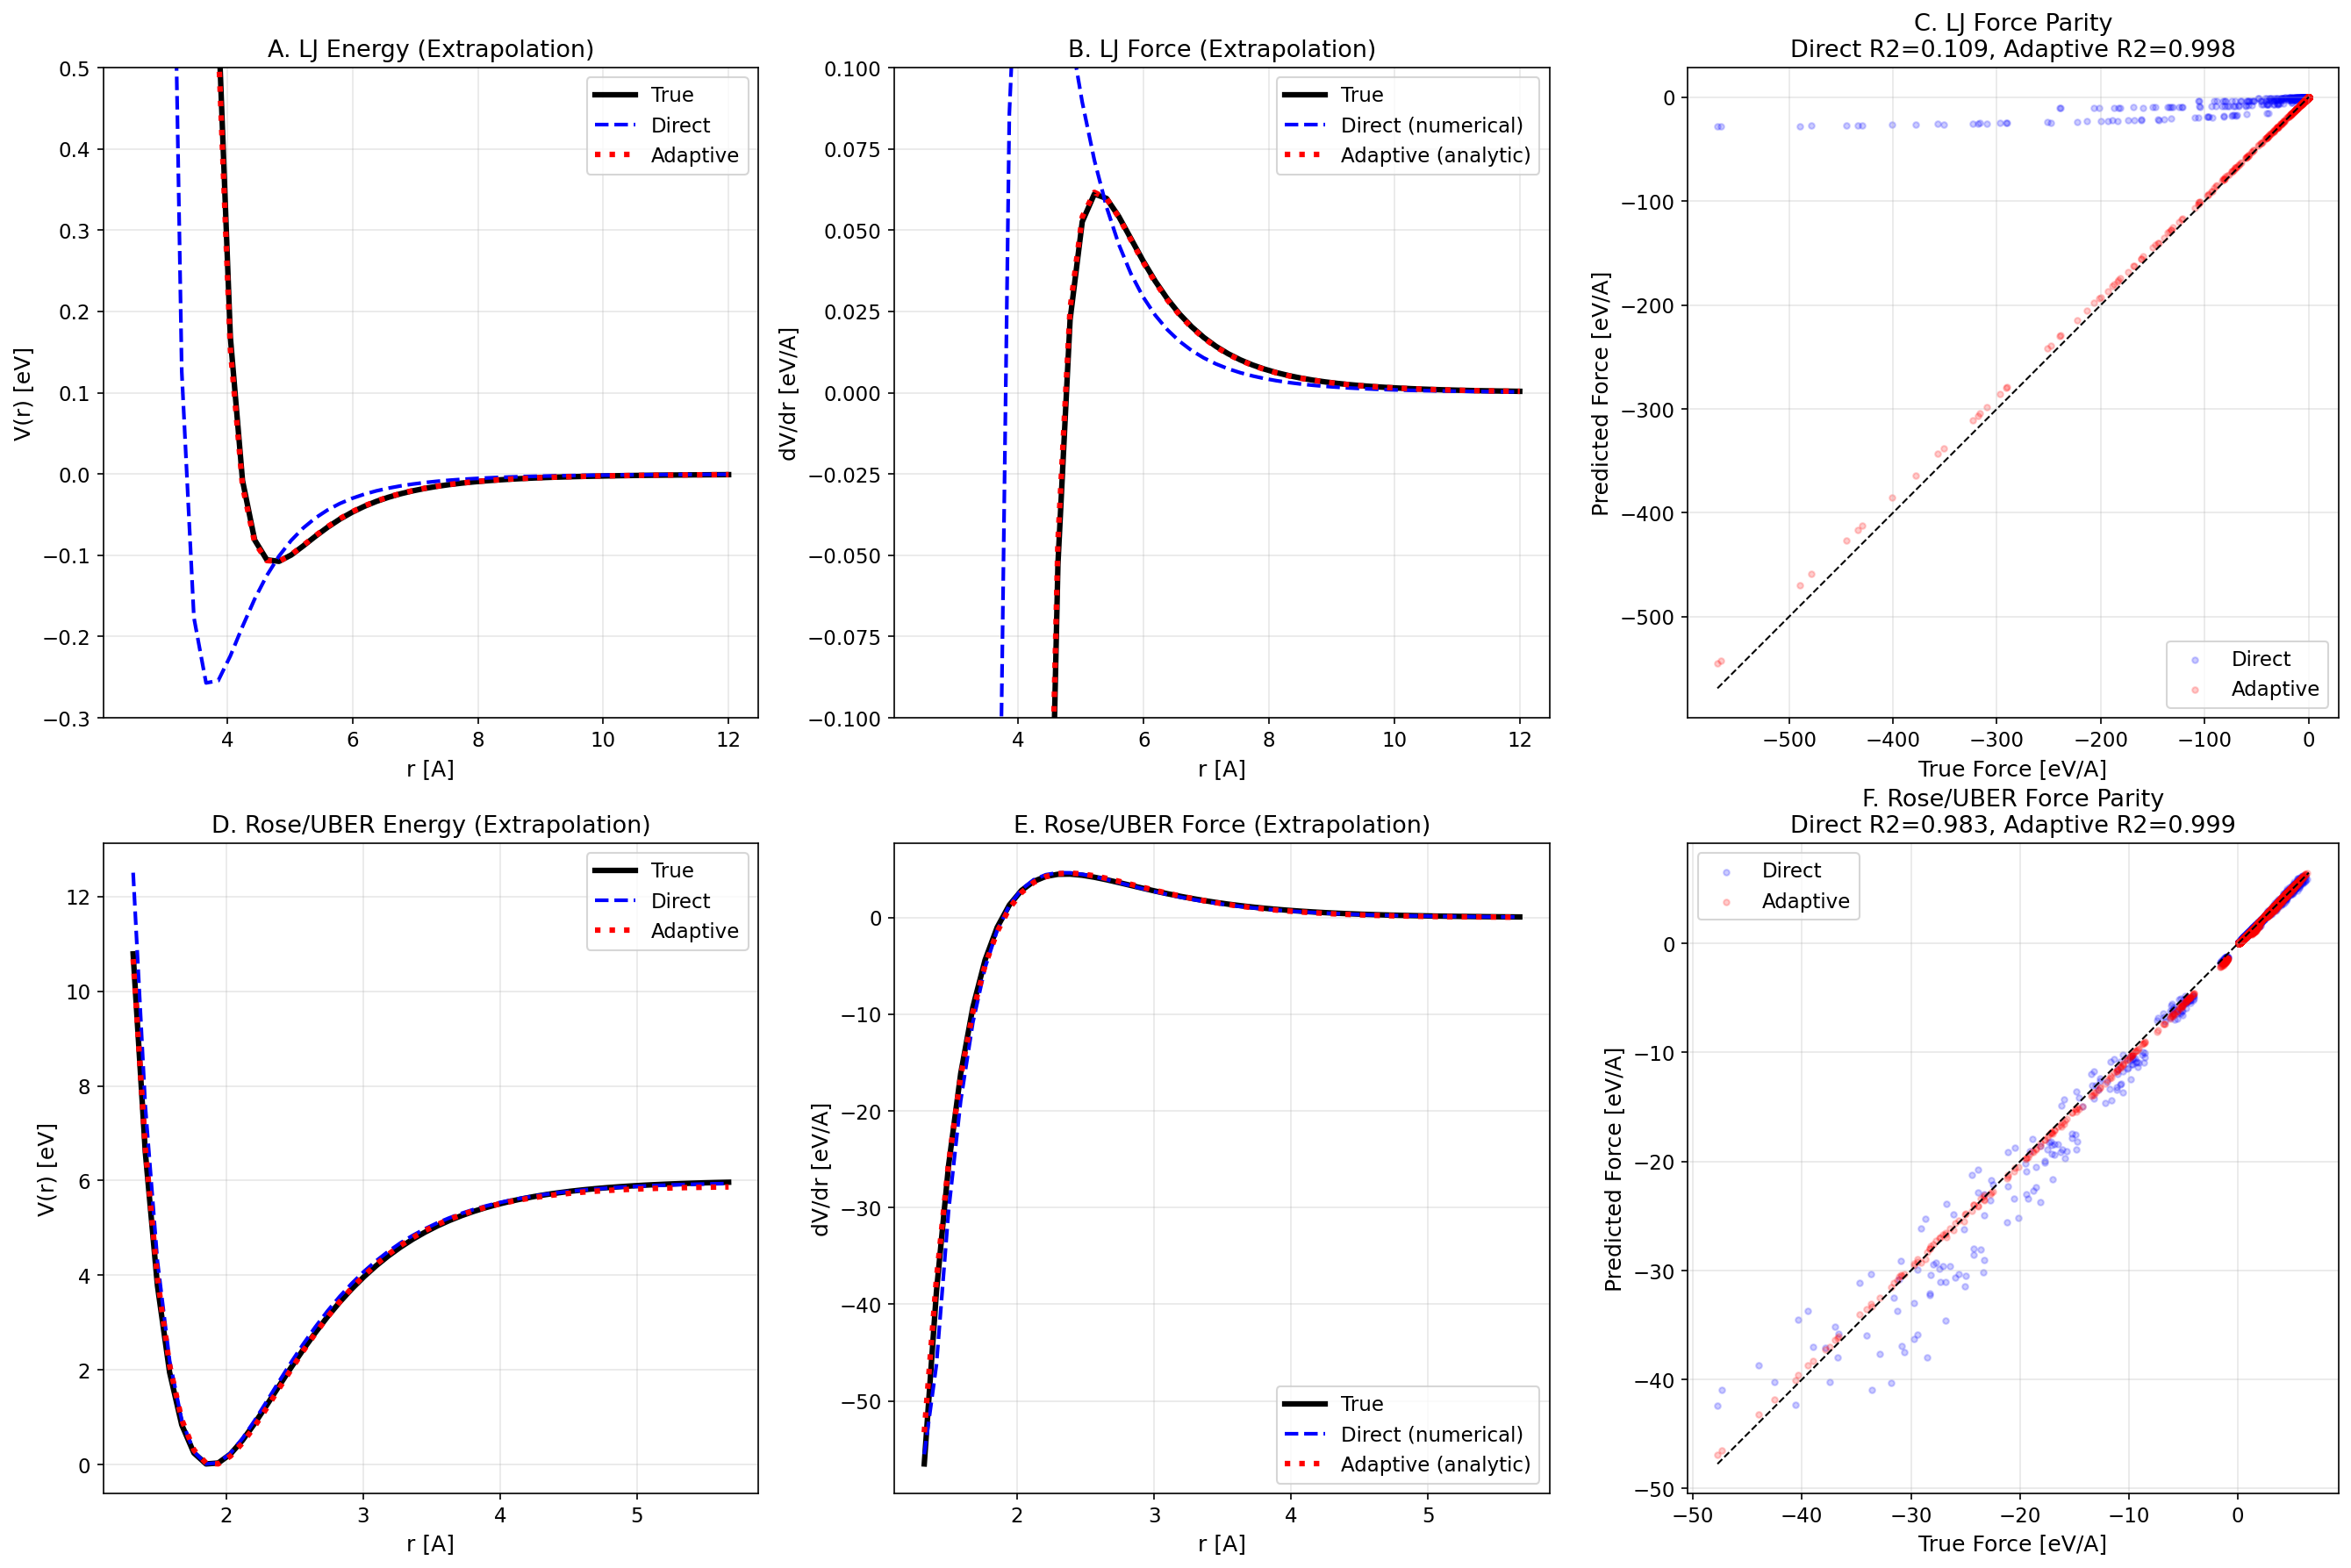
\includegraphics[width=\columnwidth]{extended/force_prediction/figures/fig_force_analysis.png}
  \caption{Force prediction comparison for extrapolation test sets ($N = 100$ training samples). (a--c)~LJ system: example energy curves, example gradients $dV/dr$, and gradient parity plot. The adaptive approach provides analytic gradients with $R^2 = 0.998$, while direct numerical differentiation yields $R^2 = 0.109$. (d--f)~Rose/UBER system: the Rose gradient approximates the true Morse gradient with $R^2 = 0.999$.}
  \label{fig:forces}
\end{figure}

Figure~\ref{fig:forces} compares force prediction quality for both systems. For the LJ system [Fig.~\ref{fig:forces}(a--c)], adaptive gradients achieve $R^2 = 0.998$ with MAE $= 0.32$~eV/\AA, while direct gradients from numerical differentiation achieve only $R^2 = 0.109$ with MAE $= 7.83$~eV/\AA---a striking contrast. Crucially, the adaptive gradient accuracy is independent of grid spacing (see Supplemental Material), whereas direct gradients degrade as the grid coarsens.

For the Rose/UBER system [Fig.~\ref{fig:forces}(d--f)], the Rose gradient closely tracks the true Morse gradient ($R^2 = 0.999$), despite the Rose equation being an approximation to the Morse potential. This demonstrates that the physics equation captures the essential shape of the force curve, not just the energy.

The force advantage extends to real DFT data. Applying the same comparison to the 28 diatomic binding curves, the adaptive approach achieves $1.46\times$ lower force MAE than direct learning for LOO (25/28 molecules favor adaptive) and $3.35\times$ lower force MAE for LGO extrapolation (13/13 molecules favor adaptive). The largest gains occur for KH ($19.0\times$) and NaH ($8.1\times$)---the same molecules where the energy advantage is greatest.

%-----------------------------------------------------------------------------
\subsection{Delta learning}
\label{sec:delta}
%-----------------------------------------------------------------------------

To combine the extrapolation advantage of the adaptive approach with the interpolation accuracy of direct learning, we implemented a delta learning strategy:
\begin{equation}
  V_\mathrm{delta}(r) = V_\mathrm{adaptive}(r;\, \hat{\boldsymbol{\theta}}) + \Delta(r;\, \mathbf{d}),
  \label{eq:delta}
\end{equation}
where $V_\mathrm{adaptive}$ is the physics-based prediction from adaptive parameters $\hat{\boldsymbol{\theta}}$, and $\Delta$ is a correction term learned by a second Ridge model from the residuals $V_\mathrm{true} - V_\mathrm{adaptive}$ on the training data.

\begin{figure*}[t]
  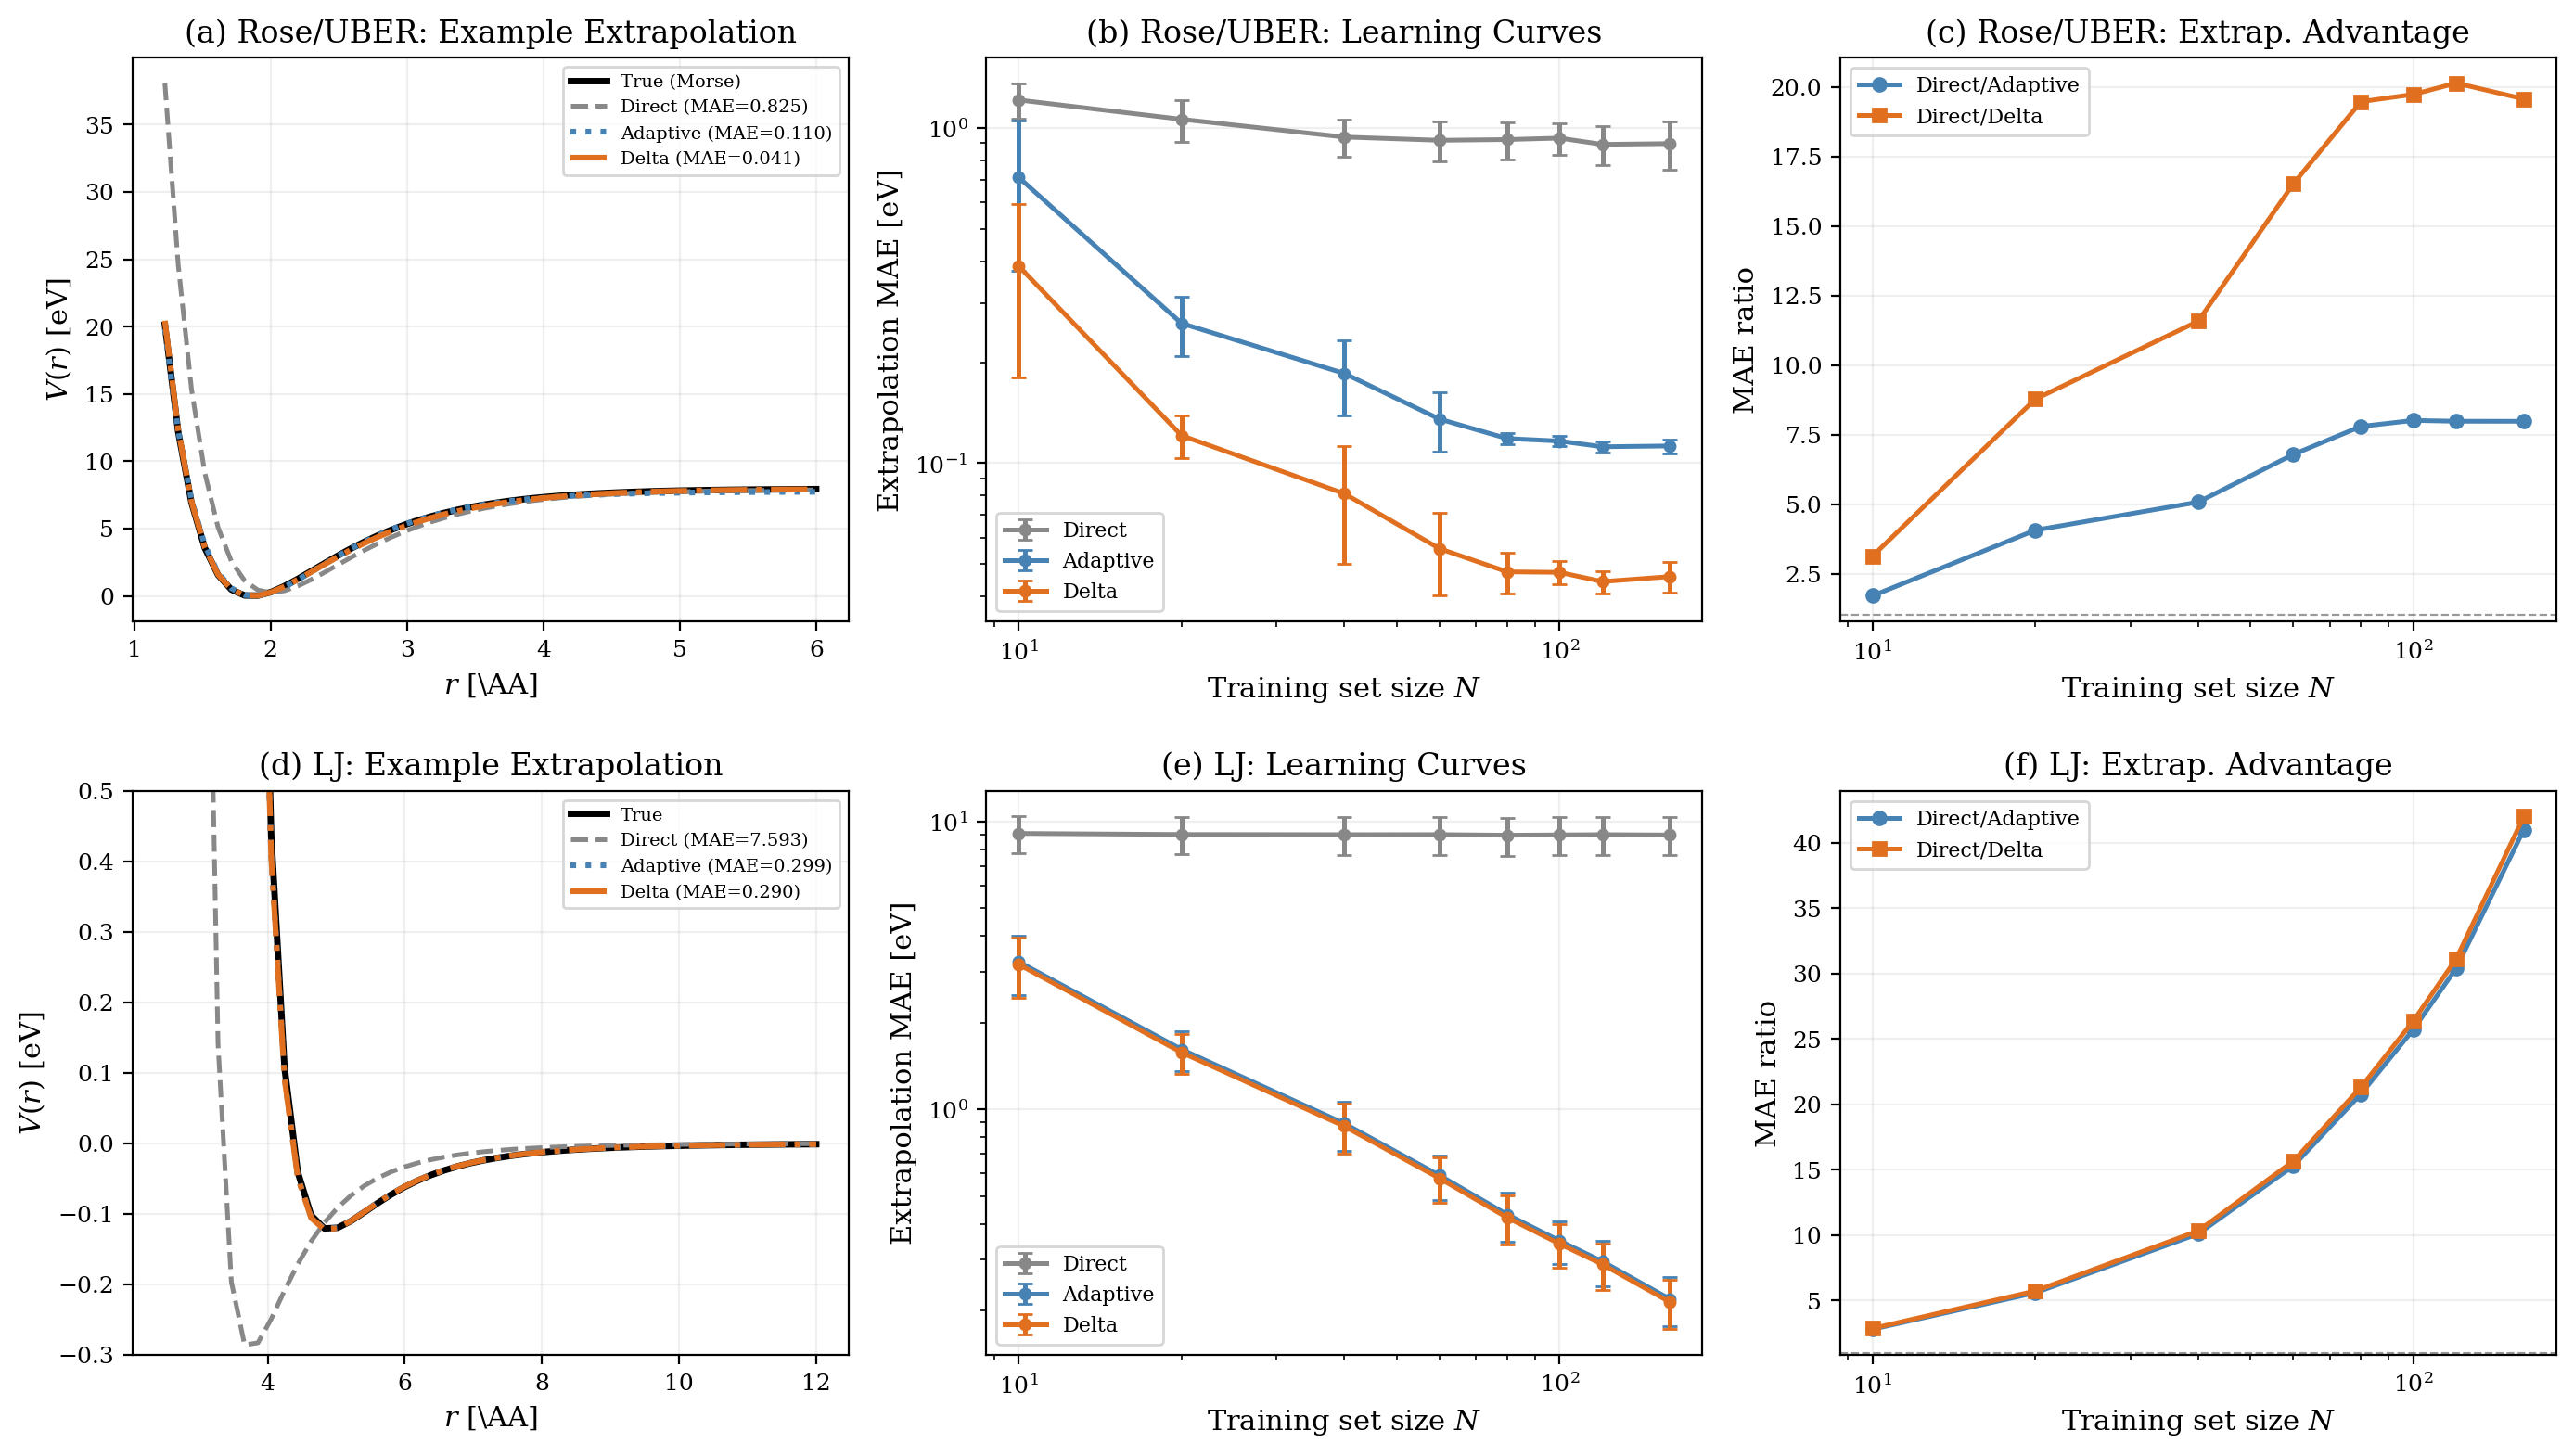
\includegraphics[width=\textwidth]{extended/delta_learning/figures/fig_delta_learning_combined.png}
  \caption{Delta learning comparison for Rose/UBER (top) and LJ (bottom) systems. (a,d)~Example extrapolation predictions showing direct (gray), adaptive (blue), and delta (orange). (b,e)~Learning curves for extrapolation MAE versus training set size. (c,f)~Ratio of direct MAE to adaptive/delta MAE (values $>1$ indicate advantage over direct). For Rose/UBER, where the physics equation is approximate, delta improves $2.7\times$ over pure adaptive. For LJ, where the physics is exact, delta provides only marginal improvement ($1.03\times$).}
  \label{fig:delta}
\end{figure*}

Figure~\ref{fig:delta} shows the three-way comparison across both systems. For the Rose/UBER system [Fig.~\ref{fig:delta}(a--c)], delta learning provides a substantial improvement over pure adaptive: at $N = 100$, the delta approach achieves MAE $= 0.041$~eV compared to $0.110$~eV for adaptive and $0.825$~eV for direct---a $2.7\times$ improvement over adaptive and $20\times$ over direct. The improvement arises because the correction term captures the systematic residual between the Rose equation and the true Morse potential ($\sim$0.02~eV fitting error), which the adaptive approach alone cannot eliminate.

For the LJ system [Fig.~\ref{fig:delta}(d--f)], delta learning provides only marginal improvement: MAE $= 0.290$~eV versus $0.299$~eV for adaptive ($1.03\times$ improvement), while both vastly outperform direct learning ($7.59$~eV, $\sim$$25\times$ worse). This contrast is expected: when the physics equation is exact, the only source of adaptive error is parameter prediction noise, which the correction term cannot systematically address.

This pattern has a clear implication: delta learning is most valuable when the physics equation provides a good but imperfect baseline. For production MLIPs, where the analytical form (e.g., Rose/UBER) will inevitably be approximate, the delta correction provides a systematic pathway to eliminate the approximation error while retaining the extrapolation advantage of the adaptive baseline.

%-----------------------------------------------------------------------------
\subsection{DFT diatomics validation}
\label{sec:dft_results}
%-----------------------------------------------------------------------------

\begin{figure}[!b]
  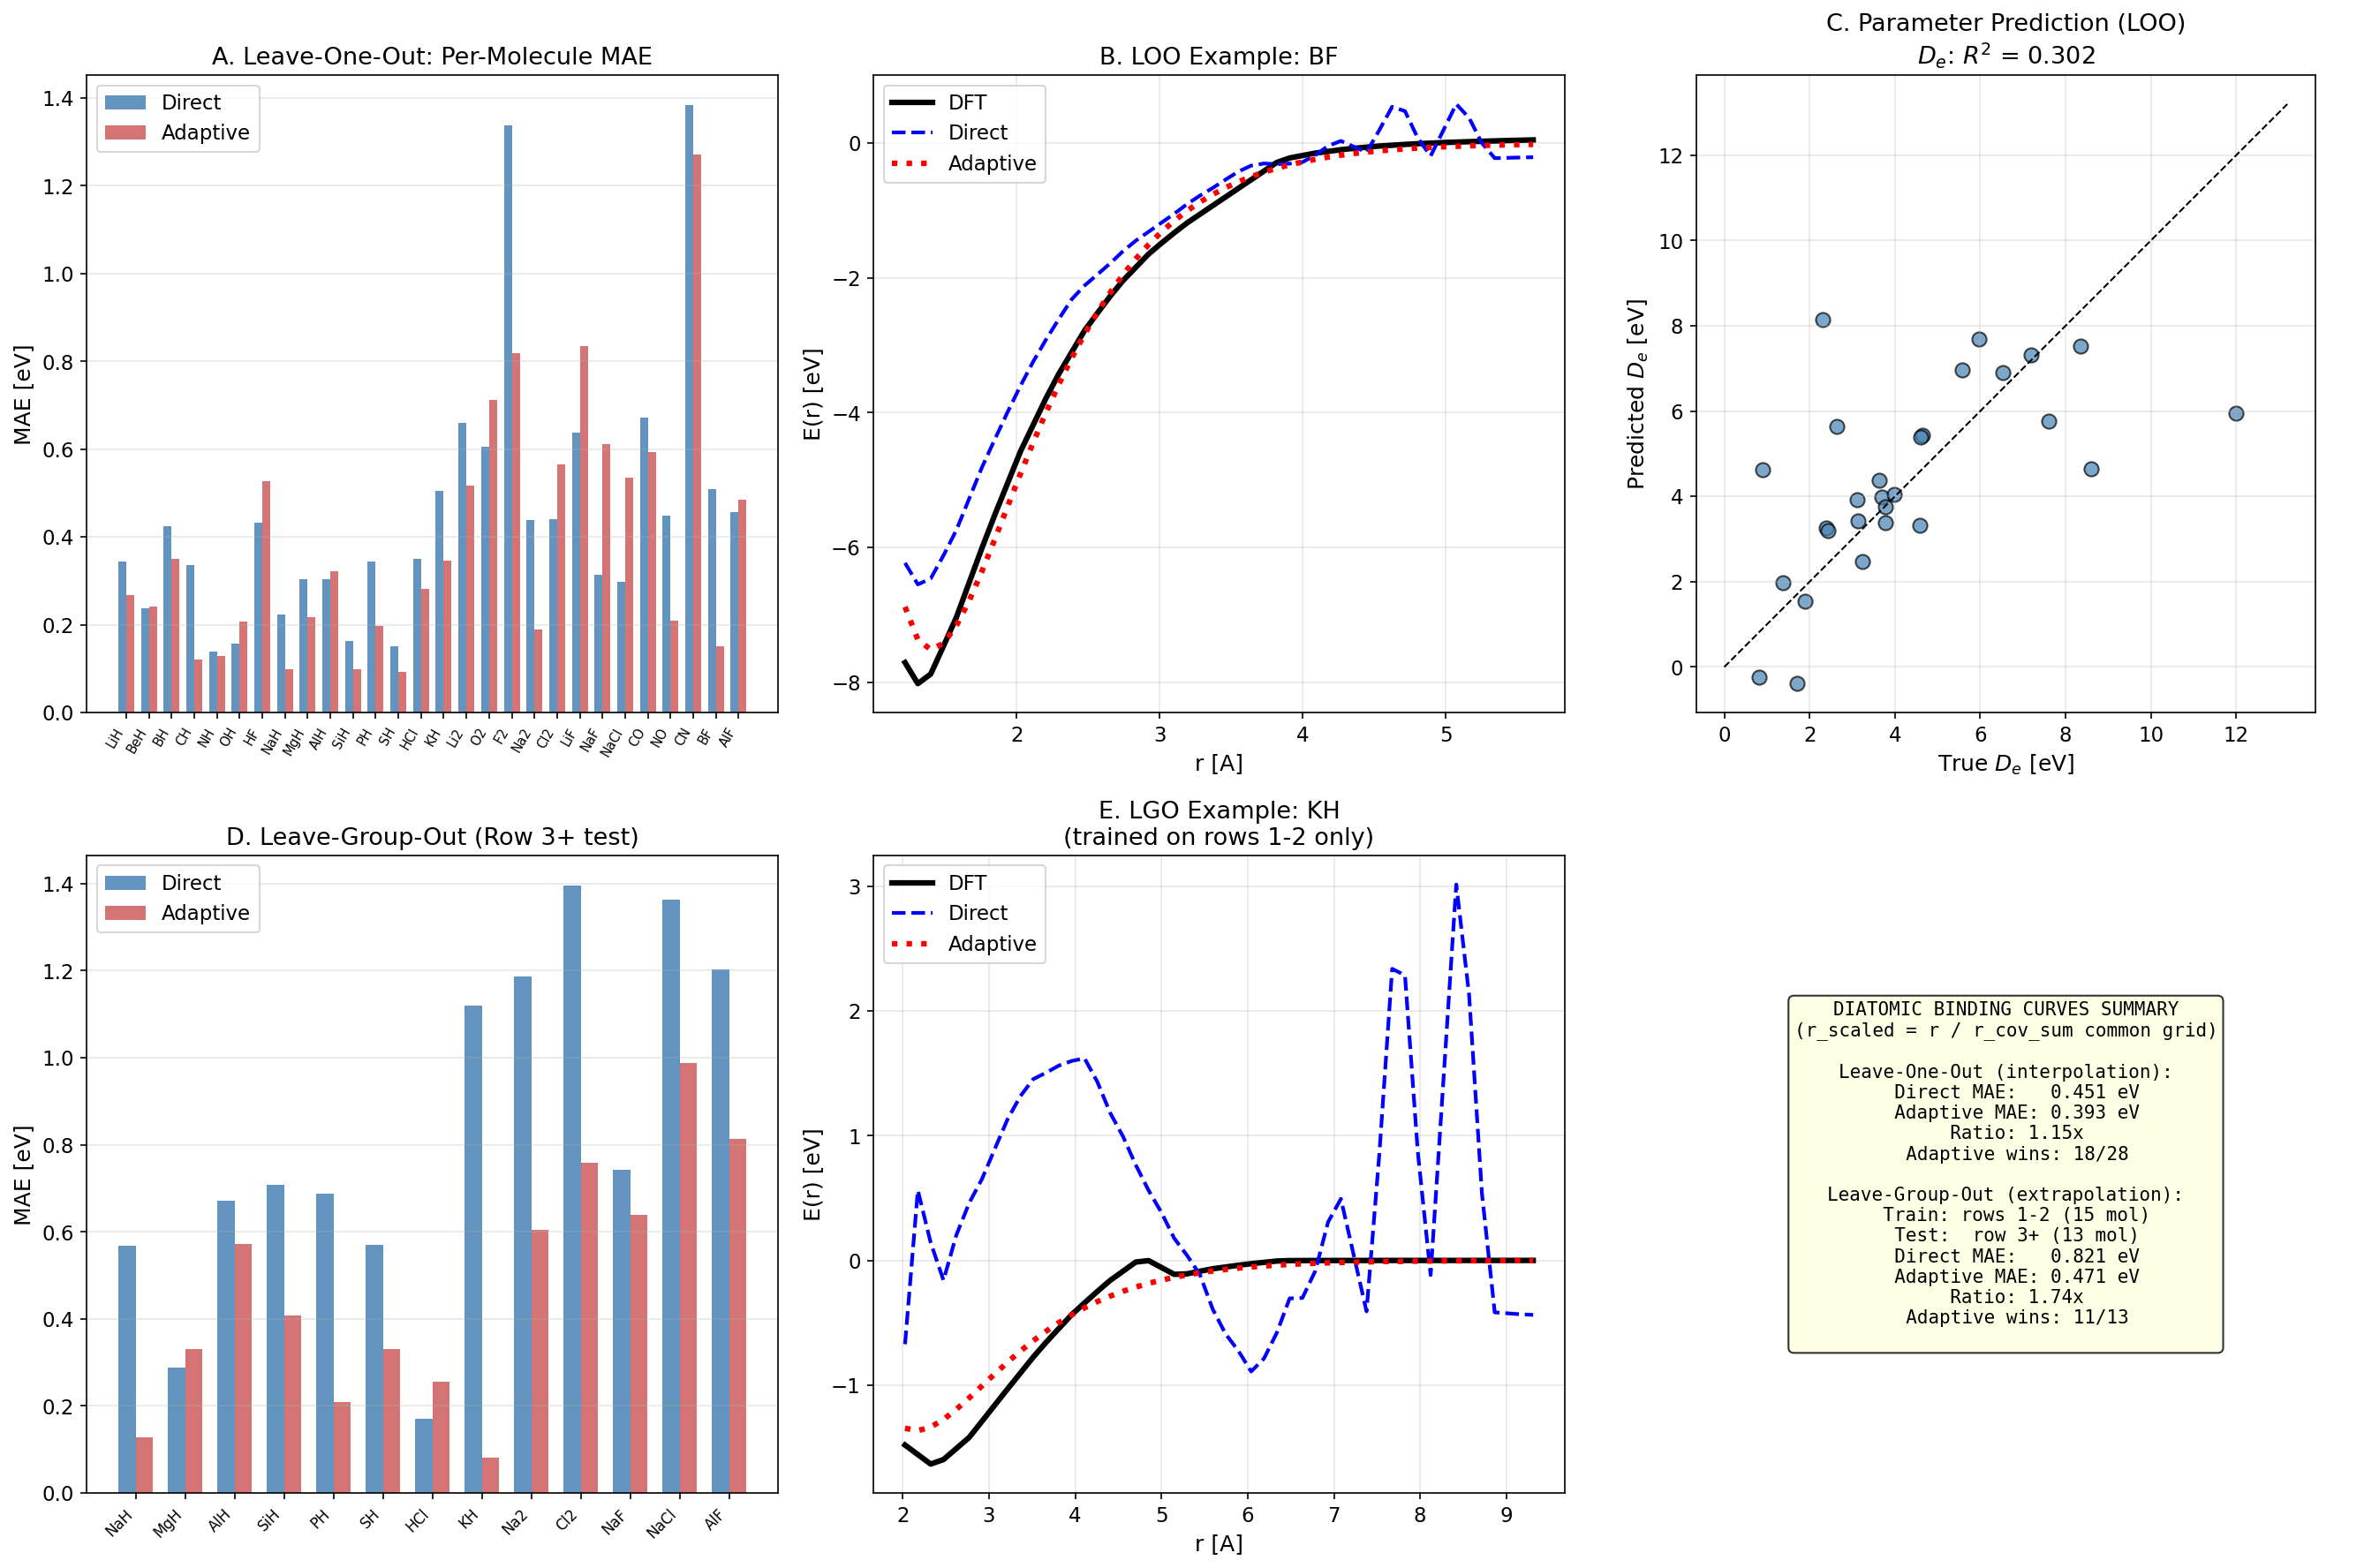
\includegraphics[width=\columnwidth]{extended/dft_diatomics/figures/fig_diatomic_comparison.png}
  \caption{DFT diatomics validation (28 molecules, PBE/def2-SVP). Top row: leave-one-out (interpolation). Bottom row: leave-group-out (extrapolation from rows 1--2 to row 3+). (a,d)~Per-molecule MAE for direct (gray) and adaptive (blue). (b)~Example LOO prediction (BF). (c)~$E_c$ parity plot. (e)~Example LGO prediction (KH, $13.8\times$ advantage). (f)~Summary statistics.}
  \label{fig:dft}
\end{figure}

\begin{table}[!b]
  \caption{Summary of extrapolation performance across all systems. The ``Delta'' column shows the delta learning MAE where applicable. DFT results use Ridge regression with 14 atomic pair descriptors and scaled radial coordinates.}
  \label{tab:summary}
  \begin{ruledtabular}
  \begin{tabular}{llcccc}
    System & Protocol & Direct & Adaptive & Delta & Ratio \\
    \hline
    Rose & Extrap.\ ($N\!=\!160$) & 0.898 & 0.113 & 0.046 & $20\times$ \\
    LJ & Extrap.\ ($N\!=\!160$) & 8.98 & 0.22 & 0.21 & $42\times$ \\
    DFT & LOO (28 mol.) & 0.451 & 0.393 & --- & $1.15\times$ \\
    DFT & LGO (13 mol.) & 0.821 & 0.471 & --- & $1.74\times$ \\
  \end{tabular}
  \end{ruledtabular}
\end{table}

Figure~\ref{fig:dft} shows the results of applying the adaptive approach to real DFT binding curves. The Rose/UBER parameters obtained from PBE/def2-SVP calculations agree reasonably with experimental values: MAE($E_c$) = 0.31~eV (consistent with PBE overbinding) and MAE($r_e$) = 0.053~\AA.

\textbf{Leave-one-out} [Fig.~\ref{fig:dft}(a--c)]: The adaptive approach achieves a mean MAE of 0.393~eV compared to 0.451~eV for direct learning, a modest $1.15\times$ advantage. The adaptive approach wins for 18 of 28 molecules. This modest improvement for interpolation is consistent with the synthetic results---when predicting within the training distribution, the advantage of physics-informed parameters is partially offset by the approximation error of the Rose equation.

\textbf{Leave-group-out} [Fig.~\ref{fig:dft}(d--f)]: The extrapolation test reveals a stronger advantage. The adaptive approach achieves a mean MAE of 0.471~eV versus 0.821~eV for direct learning---a $1.74\times$ improvement. The adaptive approach wins for 11 of 13 test molecules. The largest advantages occur for KH ($13.8\times$), NaH ($4.4\times$), and PH ($3.3\times$), all molecules where the row-3 element introduces substantially different bonding character not represented in the row 1--2 training set.

Table~\ref{tab:summary} summarizes the extrapolation performance across all three systems. The consistent pattern---adaptive advantage that grows with extrapolation severity---holds across synthetic and real data.


%=============================================================================
\section{Discussion}
\label{sec:discussion}
%=============================================================================

%-----------------------------------------------------------------------------
\subsection{Why adaptive learning works}
\label{sec:why}
%-----------------------------------------------------------------------------

The adaptive approach derives its advantage from three complementary mechanisms:

\textbf{Dimensionality reduction.} The binding energy curve $V(r)$, discretized on $N_r \sim 50$ grid points, is a high-dimensional regression target. Yet the essential physics is captured by 2--3 scaling parameters. The adaptive approach exploits this by learning the low-dimensional parameter vector instead of the full curve, effectively applying the law of corresponding states as a machine learning inductive bias.

\textbf{Smoothness and boundedness.} The scaling parameters are smooth, monotonic functions of atomic environment---$E_c$ grows with descriptor $d_1$, $\sigma$ grows with $d_1$---making them natural targets for Ridge regression. The energy curve, by contrast, varies nonlinearly with grid position and can exhibit sharp features (steep repulsive walls, inflection points) that are harder to extrapolate.

\textbf{Physics-constrained asymptotics.} Within physically meaningful parameter bounds, the analytical functional form ensures correct short-range repulsion, a well-defined minimum, and long-range decay, regardless of whether the predicted parameters are within or outside the training range. A direct model has no such constraint; its predictions at untrained grid points are unconstrained. In extrapolative regimes, direct ML models can ``hallucinate'' unphysical features---spurious oscillations, multiple minima, or divergent tails---because nothing constrains the predicted curve to resemble a valid binding potential. The adaptive approach acts as a physics-constrained approximator: the ML model may predict incorrect parameters, but the resulting potential retains the correct qualitative shape of a single-well binding curve. This is illustrated dramatically by KH under leave-group-out cross-validation, where the direct model produces a non-physical oscillatory potential (MAE = 1.12~eV) while the adaptive model maintains a smooth binding curve (MAE = 0.08~eV) despite never encountering potassium during training.

%-----------------------------------------------------------------------------
\subsection{When adaptive learning does not help}
\label{sec:limitations}
%-----------------------------------------------------------------------------

The adaptive approach introduces a systematic limitation: any error in the physics equation becomes an irreducible floor. For the Rose/UBER system, the Rose equation is an approximation to the true Morse potential, introducing a fitting residual of $\sim$0.02~eV. This is why direct learning wins for interpolation (Table~\ref{tab:learning_curves}, $0.40\times$ ratio): within the training distribution, direct learning can achieve lower error than the physics equation allows.

This limitation vanishes when the physics equation is exact. For the Lennard-Jones system, the adaptive approach dominates even for interpolation ($63\times$ advantage), because no approximation error exists. For real DFT data, the Rose equation is an approximation of variable quality---some molecules (e.g., homonuclear diatomics, hydrides) fit well (RMSE $< 0.1$~eV), while others (ionic molecules, multi-reference systems) fit poorly.

As demonstrated in Sec.~\ref{sec:delta}, the delta learning strategy effectively addresses this limitation: the correction term captures the systematic residual between the analytical form and the true potential, reducing the error floor by $2.7\times$ for Rose/UBER while preserving the extrapolation advantage. Importantly, delta learning provides maximal benefit precisely when the physics equation is approximate---confirming that the approach is most useful in the regime where it is most needed.

%-----------------------------------------------------------------------------
\subsection{Model capacity versus physics}
\label{sec:capacity}
%-----------------------------------------------------------------------------

A natural question is whether the adaptive advantage reflects the physics equation or merely the low dimensionality of the parameter space---or, equivalently, whether a sufficiently expressive direct model could match the adaptive approach. We tested this in two ways.

First, we compared against direct learning with polynomial feature expansion of increasing degree for the LJ system (extrapolation regime, $N = 100$). As shown in Table~\ref{tab:polynomial}, even degree-6 polynomials (27 features) cannot match the adaptive approach (2 features + physics): MAE = 0.67~eV versus 0.39~eV, despite using $13.5\times$ more parameters.

Second, we replaced Ridge regression with multilayer perceptrons (MLPs) as direct nonlinear baselines ($N = 160$, 5 random seeds), sweeping over 7 architectures (2--4 hidden layers, 32--256 neurons) and 4 activation functions (ReLU, tanh, sigmoid, SiLU)---56 configurations in total. For the LJ system, the best MLP (SiLU activation) achieves MAE = $7.76 \pm 0.46$~eV, an 8\% improvement over direct Ridge ($8.42 \pm 0.48$~eV) but still $39\times$ worse than adaptive Ridge ($0.20 \pm 0.01$~eV). For Rose/UBER, the best direct MLP (SiLU, MAE = $0.19 \pm 0.01$~eV) performs comparably to direct Ridge ($0.18 \pm 0.02$~eV); all other activations perform substantially worse, as the MLPs overfit to the training domain and extrapolate less reliably than a global linear model. In both systems, adaptive Ridge remains the clear winner ($0.07 \pm 0.001$~eV for Rose/UBER). These results confirm that the adaptive advantage stems from the correct functional form, not from model capacity, activation function choice, or the linear-versus-nonlinear distinction. Full architecture and activation comparisons are provided in the Supplemental Material.

%-----------------------------------------------------------------------------
\subsection{Connection to aPBE0}
\label{sec:apbe0}
%-----------------------------------------------------------------------------

Our results confirm that the principle underlying aPBE0---learning bounded, smooth parameters for a known physics equation rather than the output quantity directly---is general and operates at multiple scales. In aPBE0, the ML model learns the exchange mixing parameter $\alpha \in [0, 1]$, and the hybrid functional $E_\mathrm{xc} = (1-\alpha)E_\mathrm{PBE} + \alpha E_\mathrm{HF}$ provides the physics. Here, the ML model learns $(E_c, r_e, l)$ or $(\varepsilon, \sigma)$, and the Rose or LJ equation provides the physics. In both cases, the key ingredients are:
\begin{enumerate}
  \item A well-motivated analytical functional form;
  \item Bounded, smooth parameters as regression targets;
  \item Physics-guaranteed extrapolation behavior.
\end{enumerate}

This suggests a general design principle for physics-informed machine learning: whenever a known equation connects a small number of interpretable parameters to the quantity of interest, learning the parameters is preferable to learning the quantity directly.

%-----------------------------------------------------------------------------
\subsection{Toward production machine learning potentials}
\label{sec:outlook}
%-----------------------------------------------------------------------------

The present study demonstrates the principle on pair potentials with simple descriptors. Several extensions are needed for production applications:

\textbf{Atomic environment descriptors.} The 2D synthetic descriptors and 14-dimensional atomic pair features used here should be replaced by proper many-body descriptors such as SOAP~\cite{Bartok2010,Musil2021} or ACE~\cite{Drautz2019}, which provide a complete representation of the local atomic environment.

\textbf{Many-body potentials.} The Rose/UBER equation describes pair interactions. For many-body systems, adaptive parameters could be incorporated into embedded-atom models or other many-body frameworks, where the embedding function or pair functional is parameterized by learnable quantities.

\textbf{Delta learning at scale.} The delta learning strategy demonstrated in Sec.~\ref{sec:delta} provides a practical pathway for production systems, where the analytical form will inevitably be approximate. Combining adaptive parameter prediction with a learned correction term retains the extrapolation advantage while eliminating the physics equation's approximation error.

\textbf{Neural network models.} Replacing Ridge regression with neural networks would enable learning nonlinear descriptor-to-parameter mappings, potentially capturing more complex relationships while retaining the physics equation as an output layer.

\textbf{Analytical forces.} As shown in Sec.~\ref{sec:forces}, the adaptive approach provides analytical, grid-independent forces for free---a practical advantage for molecular dynamics applications where force accuracy is critical. This benefit extends naturally to production architectures: any differentiable physics equation yields analytical forces via automatic differentiation.


%=============================================================================
\section{Conclusions}
\label{sec:conclusions}
%=============================================================================

We have demonstrated that machine learning interatomic potentials can achieve substantially better extrapolation by learning universal scaling parameters instead of energies directly. The adaptive approach---predicting Rose/UBER parameters $(E_c, r_e, l)$ or Lennard-Jones parameters $(\varepsilon, \sigma)$ from descriptors, then reconstructing the potential via the known physics equation---yields $2.3\times$ to $42\times$ lower extrapolation error on synthetic systems and $1.74\times$ on real DFT diatomic binding curves. The approach provides analytical forces at no additional cost, and a delta learning extension that corrects for the physics equation's approximation error yields a further $2.7\times$ improvement.

The advantage is rooted in a principle shared with the adaptive density functional aPBE0~\cite{Khan2025}: whenever a known equation connects a small number of bounded, smooth parameters to the quantity of interest, learning the parameters is preferable to learning the quantity directly. The analytical form provides correct asymptotic behavior, the low-dimensional parameter space reduces the regression burden, and the smoothness of the parameters facilitates generalization.

More broadly, this work and aPBE0 together point toward a ``gray-box'' strategy for scientific machine learning. Rather than replacing physical models with black-box approximators (neural networks, kernel methods), or constraining oneself to white-box analytical theory, the adaptive approach retains the rigorous functional forms of physics while offloading system-specific complexity to the machine learning model. The physics equation provides the guardrails---correct asymptotics, conservation laws, interpretable parameters---while the ML model provides the flexibility to adapt across chemical space. That this strategy operates successfully across scales, from exchange-correlation functionals to interatomic potentials, suggests it may generalize to other domains of computational chemistry where known analytical forms exist.

The present results establish the adaptive approach on pair potentials. Extending to many-body systems with production-quality atomic environment descriptors is a natural next step toward practical applications.


%=============================================================================
\begin{acknowledgments}
We thank the Digital Research Alliance of Canada (formerly Compute Canada) for computational resources. This work was supported by [funding information to be added].
\end{acknowledgments}
%=============================================================================

\bibliography{references}


%=============================================================================
% SUPPLEMENTAL MATERIAL
%=============================================================================
\clearpage
\onecolumngrid
\appendix

\section{Detailed walkthrough of the experimental design}
\label{app:walkthrough}

This appendix provides a concrete, step-by-step description of the synthetic experiments for readers unfamiliar with the setup.

\subsection{Descriptors and their physical meaning}

The synthetic descriptors $\mathbf{d} = (d_1, d_2)$ serve as proxies for local atomic environment features. In production MLIPs, these would be many-body descriptors such as SOAP~\cite{Bartok2010} or ACE~\cite{Drautz2019} vectors, which encode the positions and species of neighboring atoms. Here, two scalar descriptors suffice to parameterize a family of pair potentials:
\begin{center}
\begin{tabular}{lll}
  \toprule
  & LJ system & Rose/UBER system \\
  \midrule
  $d_1$ controls & size: $\sigma = 2.5 + 0.5\,d_1$ [\AA] & bond strength: $D_e = 0.5 + 2.0\,d_1$ [eV] \\
  $d_2$ controls & well depth: $\varepsilon = 0.05 + 0.1\,d_2$ [eV] & bond length: $r_e = 1.5 + 0.5\,d_2$ [\AA] \\
  \bottomrule
\end{tabular}
\end{center}
These linear mappings are unknown to the ML model---it must learn the relationship between descriptors and potential parameters (or potential curves) from training examples alone.

\subsection{What ``extrapolation'' means}

The training and test sets occupy non-overlapping regions of descriptor space:
\begin{center}
\begin{tabular}{lll}
  \toprule
  & Training & Extrapolation test \\
  \midrule
  $d_1$ range & $[0.5,\; 1.5]$ & $[2.5,\; 4.0]$ \\
  $d_2$ range & $[0.5,\; 1.5]$ & $[0.5,\; 1.5]$ \\
  LJ $\sigma$ range & $[2.75,\; 3.25]$ \AA & $[3.75,\; 4.50]$ \AA \\
  Rose $D_e$ range & $[1.5,\; 3.5]$ eV & $[5.5,\; 8.5]$ eV \\
  \bottomrule
\end{tabular}
\end{center}
The test systems have larger atoms (LJ) or stronger bonds (Rose) than anything in the training set. This is analogous to training an MLIP on first- and second-row elements and testing on third-row elements, which is exactly the protocol used in the DFT diatomics validation (Sec.~\ref{sec:dft}).

\subsection{How each approach processes the same input}

Consider a specific LJ test point: $d_1 = 3.0$, $d_2 = 1.0$, corresponding to $\sigma = 4.0$~\AA, $\varepsilon = 0.15$~eV. The true potential is $V(r) = 4 \times 0.15 \times [(4.0/r)^{12} - (4.0/r)^6]$. All approaches receive the same input $(d_1, d_2) = (3.0, 1.0)$:

\textbf{Direct learning} (Ridge or MLP): The model has learned a mapping $\mathbf{d} \to \{V(r_i)\}_{i=1}^{50}$ from training examples where $d_1 \in [0.5, 1.5]$. At $d_1 = 3.0$, it must extrapolate this mapping. Because the potential energy $V(r_i)$ depends on $d_1$ through $\sigma^{12}$ and $\sigma^6$---highly nonlinear functions---neither a linear model (Ridge) nor a neural network (MLP, which has only seen $d_1 \leq 1.5$) can reliably predict the curve. The result is a physically meaningless prediction with MAE $\sim 8$~eV.

\textbf{Adaptive learning} (Ridge): The model has learned a mapping $\mathbf{d} \to (\varepsilon, \sigma)$. Since both $\varepsilon$ and $\sigma$ depend \emph{linearly} on the descriptors, a linear model extrapolates correctly: $\hat{\sigma} \approx 4.0$~\AA, $\hat{\varepsilon} \approx 0.15$~eV. The physics equation $V = 4\varepsilon[(\sigma/r)^{12} - (\sigma/r)^6]$ then produces the correct curve analytically. MAE $\sim 0.2$~eV.

The critical point is that the hard nonlinearity---$(\sigma/r)^{12}$---resides in the \emph{physics equation}, not in the descriptor-to-parameter mapping. The adaptive approach delegates this nonlinearity to the known equation, while the direct approach asks the ML model to learn it from data.

\subsection{Role of the linear descriptor-to-parameter mapping}

The synthetic experiments use linear descriptor-to-parameter mappings by design: this ensures that the only difference between direct and adaptive is the physics equation, providing a clean controlled comparison. This linearity does not trivialize the problem for the direct approach, because the energy $V(r_i)$ at any fixed grid point depends nonlinearly on $\sigma$ (through $\sigma^{12}$), so the descriptor-to-\emph{energy} mapping is strongly nonlinear even when the descriptor-to-\emph{parameter} mapping is linear.

For the DFT diatomics (Sec.~\ref{sec:dft}), the descriptor-to-parameter relationship is genuinely nonlinear and unknown: the mapping from atomic numbers, electronegativities, and covalent radii to Rose parameters $(E_c, r_e, l)$ is non-trivial. The adaptive approach still outperforms direct learning ($1.74\times$ for extrapolation), confirming that the advantage extends beyond the linear-mapping case.


\section{Polynomial feature analysis}
\label{app:polynomial}

To test whether the adaptive advantage reflects the physics equation or merely model capacity, we compared adaptive learning against direct learning with polynomial feature expansion of increasing degree on the LJ system (extrapolation regime, $N = 100$ training samples).

\begin{table}[h]
  \caption{Extrapolation MAE for direct learning with polynomial features versus adaptive learning (LJ system, $N = 100$).}
  \label{tab:polynomial}
  \begin{ruledtabular}
  \begin{tabular}{cccc}
    Poly.\ degree & No.\ features & Direct MAE (eV) & vs.\ Adaptive (0.39~eV) \\
    \hline
    1 (linear) & 2 & 9.63 & $24.8\times$ worse \\
    2 & 5 & 8.79 & $22.6\times$ worse \\
    3 & 9 & 7.42 & $19.1\times$ worse \\
    4 & 14 & 5.68 & $14.6\times$ worse \\
    5 & 20 & 3.24 & $8.3\times$ worse \\
    6 & 27 & 0.67 & $1.7\times$ worse \\
  \end{tabular}
  \end{ruledtabular}
\end{table}

Even degree-6 polynomials (27 features) cannot match the adaptive approach (2 linear features $+$ LJ physics). For interpolation, degree 5--6 polynomials do match adaptive, confirming that the advantage is specifically about extrapolation physics. At $N = 5000$ training samples, direct learning with degree-4 polynomials still achieves MAE $= 3.77$~eV versus adaptive MAE $= 0.006$~eV.


\section{Force prediction: grid spacing sensitivity}
\label{app:forces}

As discussed in Sec.~\ref{sec:forces}, the adaptive approach provides analytical, grid-independent forces. To quantify the grid dependence of the direct approach, we evaluated LJ force prediction accuracy as a function of grid spacing ($N_r \in \{10, 20, 30, 50, 100, 200\}$ points over $r \in [2.5, 12.0]$~\AA).

The adaptive force MAE is essentially constant across all grid spacings (since forces are computed analytically from Eq.~\eqref{eq:lj_force}), while the direct force MAE increases monotonically as the grid coarsens---both from reduced numerical differentiation accuracy and from the direct energy prediction being evaluated at fewer points. At the coarsest grid ($N_r = 10$, $\mathrm{d}r = 1.06$~\AA), the direct force MAE is $\sim$$10\times$ worse than at the finest grid ($N_r = 200$, $\mathrm{d}r = 0.048$~\AA), while the adaptive approach is unaffected.


\section{MLP nonlinear baseline}
\label{app:mlp}

To verify that the adaptive advantage is not an artifact of comparing a physics-nonlinear model against a linear baseline, we tested direct and adaptive learning with multilayer perceptrons (MLPs). A comprehensive sweep was performed over 7 architectures (2--4 hidden layers with 32--256 neurons) and 4 activation functions (ReLU, tanh, sigmoid, SiLU/Swish), totaling 56 MLP configurations tested in both the direct and adaptive pathways. Sklearn's \texttt{MLPRegressor} was used for ReLU, tanh, and sigmoid; PyTorch was used for SiLU. All MLPs used adaptive learning rate, early stopping (validation fraction 0.15, patience 20), and L2 regularization ($\alpha = 0.001$).

\begin{table}[h]
  \caption{Extrapolation MAE (eV) at $N = 160$ for direct Ridge, best direct MLP (across 28 architecture/activation combinations), and adaptive Ridge, averaged over 5 random seeds.}
  \label{tab:mlp}
  \begin{ruledtabular}
  \begin{tabular}{lcccc}
    System & Direct Ridge & Best Direct MLP & Adaptive Ridge & Ratio \\
    \hline
    LJ         & $8.42 \pm 0.48$ & $7.76 \pm 0.46$\textsuperscript{a} & $\mathbf{0.20 \pm 0.01}$ & $39\times$ \\
    Rose/UBER  & $0.18 \pm 0.02$ & $0.19 \pm 0.01$\textsuperscript{b} & $\mathbf{0.07 \pm 0.001}$ & $2.7\times$ \\
  \end{tabular}
  \end{ruledtabular}
  \textsuperscript{a}SiLU, (128,64). \textsuperscript{b}SiLU, (256,128).
\end{table}

SiLU consistently outperformed other activations for the direct pathway, while tanh and sigmoid performed substantially worse than even linear Ridge for extrapolation. For the LJ system, the best MLP improves over Ridge by only 8\%, confirming that the direct approach's failure is not due to insufficient model capacity or activation choice but to the fundamental difficulty of extrapolating $V(r;\sigma)$ without the physics equation. For the Rose/UBER system, only SiLU MLPs match Ridge; all other activations degrade performance due to overfitting to the training domain. In both cases, adaptive Ridge with only 2--3 physics parameters dominates all 56 direct MLP configurations.


\section{Ridge versus kernel ridge regression}
\label{app:krr}

Kernel ridge regression (KRR) with RBF kernel was tested as an alternative to Ridge regression for both approaches. In the extrapolation regime, KRR yields identical performance for direct and adaptive approaches: both converge to $\sim$3.2~eV MAE with no improvement as training set size increases. This occurs because the RBF kernel $K(\mathbf{x}, \mathbf{x}') = \exp(-\gamma\|\mathbf{x} - \mathbf{x}'\|^2)$ decays to zero for test points far from training data, causing predictions to regress toward the training mean. While alternative kernel choices (e.g., polynomial or linear kernels) or physics-informed feature engineering could mitigate this behavior, Ridge regression provides a transparent global linear baseline that isolates the structural effect of the adaptive approach without confounding kernel selection.


\section{DFT diatomics: per-molecule results}
\label{app:dft_details}

Table~\ref{tab:dft_loo} shows the full leave-one-out results for all 28 molecules, and Table~\ref{tab:dft_lgo} shows the leave-group-out results.

\begin{table}[h]
  \caption{Leave-one-out cross-validation: per-molecule MAE (eV) for 28 DFT diatomics, sorted by adaptive advantage (ratio).}
  \label{tab:dft_loo}
  \begin{ruledtabular}
  \begin{tabular}{lcccc}
    Molecule & Direct MAE & Adaptive MAE & Ratio & Winner \\
    \hline
    BF   & 0.509 & 0.151 & 3.37 & Adaptive \\
    Na2  & 0.438 & 0.189 & 2.32 & Adaptive \\
    CH   & 0.336 & 0.121 & 2.78 & Adaptive \\
    NO   & 0.448 & 0.210 & 2.14 & Adaptive \\
    PH   & 0.345 & 0.198 & 1.74 & Adaptive \\
    NaH  & 0.223 & 0.099 & 2.25 & Adaptive \\
    SH   & 0.151 & 0.092 & 1.64 & Adaptive \\
    SiH  & 0.162 & 0.099 & 1.64 & Adaptive \\
    KH   & 0.505 & 0.346 & 1.46 & Adaptive \\
    MgH  & 0.305 & 0.217 & 1.40 & Adaptive \\
    Li2  & 0.659 & 0.518 & 1.27 & Adaptive \\
    LiH  & 0.345 & 0.267 & 1.29 & Adaptive \\
    HCl  & 0.350 & 0.281 & 1.24 & Adaptive \\
    NH   & 0.139 & 0.129 & 1.08 & Adaptive \\
    CO   & 0.672 & 0.594 & 1.13 & Adaptive \\
    CN   & 1.383 & 1.272 & 1.09 & Adaptive \\
    BH   & 0.424 & 0.351 & 1.21 & Adaptive \\
    AlH  & 0.305 & 0.323 & 0.94 & Direct \\
    BeH  & 0.238 & 0.242 & 0.98 & Direct \\
    AlF  & 0.458 & 0.485 & 0.94 & Direct \\
    NaCl & 0.299 & 0.535 & 0.56 & Direct \\
    NaF  & 0.313 & 0.611 & 0.51 & Direct \\
    HF   & 0.432 & 0.527 & 0.82 & Direct \\
    Cl2  & 0.442 & 0.566 & 0.78 & Direct \\
    OH   & 0.156 & 0.207 & 0.76 & Direct \\
    O2   & 0.605 & 0.712 & 0.85 & Direct \\
    F2   & 1.337 & 0.819 & 1.63 & Adaptive \\
    LiF  & 0.639 & 0.834 & 0.77 & Direct \\
    \hline
    \textbf{Mean} & \textbf{0.451} & \textbf{0.393} & $\mathbf{1.15\times}$ & 18/28 \\
  \end{tabular}
  \end{ruledtabular}
\end{table}

\begin{table}[h]
  \caption{Leave-group-out cross-validation: per-molecule MAE (eV) for 13 test molecules (row 3+ atoms), sorted by adaptive advantage.}
  \label{tab:dft_lgo}
  \begin{ruledtabular}
  \begin{tabular}{lcccc}
    Molecule & Direct MAE & Adaptive MAE & Ratio & Winner \\
    \hline
    KH   & 1.120 & 0.081 & 13.84 & Adaptive \\
    NaH  & 0.567 & 0.128 & 4.44 & Adaptive \\
    PH   & 0.688 & 0.210 & 3.28 & Adaptive \\
    Na2  & 1.187 & 0.605 & 1.96 & Adaptive \\
    Cl2  & 1.395 & 0.759 & 1.84 & Adaptive \\
    SiH  & 0.708 & 0.408 & 1.74 & Adaptive \\
    SH   & 0.571 & 0.332 & 1.72 & Adaptive \\
    AlF  & 1.203 & 0.814 & 1.48 & Adaptive \\
    NaCl & 1.363 & 0.987 & 1.38 & Adaptive \\
    AlH  & 0.672 & 0.571 & 1.18 & Adaptive \\
    NaF  & 0.744 & 0.639 & 1.16 & Adaptive \\
    MgH  & 0.289 & 0.330 & 0.88 & Direct \\
    HCl  & 0.170 & 0.255 & 0.67 & Direct \\
    \hline
    \textbf{Mean} & \textbf{0.821} & \textbf{0.471} & $\mathbf{1.74\times}$ & 11/13 \\
  \end{tabular}
  \end{ruledtabular}
\end{table}

\end{document}
